\setcounter{page}{1}


\counterwithin{table}{section}
\counterwithin{figure}{section}

\section{Matryoshka Kernel Layer Algorithms}
\label{mkl_algos}
%对于我们的MKL~\ref{subsec:mk}，其算法的伪代码如Algo.~ref{alg:adaptive_input_conv_slice}和~ref{alg:adaptive_output_conv_slice}所示。对于我们的SSA模型,我们在Matryoshka Kernel Input Layer和Matryoshka Kernel Output Layer都是用的大小为3x3的卷积核，stride、dilation、groups均为1，可以注意到我们的MKL输入输出空间大小不变。
The pseudocode for our proposed Matryoshka Kernel Layer (MKL), as detailed in \S\ref{subsec:mk}, is presented in Algo.~\ref{alg:adaptive_input_conv_slice} and Algo.~\ref{alg:adaptive_output_conv_slice}. 
In our SSA model, both the Matryoshka Kernel Input and Output Layers utilize a $3 \times 3$ convolution kernel. 
The stride, dilation, and groups are all set to 1. 
Consequently, the spatial dimensions of the input and output feature maps remain unchanged across the MKL operations.

\begin{algorithm}
\caption{Matryoshka Kernel Input Layer Forward Pass}
\label{alg:adaptive_input_conv_slice}
\begin{algorithmic}[1]

\REQUIRE
\INPUT $\mathbf{X} \in \mathbb{R}^{N \times C_{\text{in}} \times H \times W}$
\INPUT Nested convolution weight 
$\mathbf{W}_{\text{nested}} \in \mathbb{R}^{D \times C_{\text{max}} \times k \times k}$
\INPUT Convolution bias $\mathbf{b} \in \mathbb{R}^{D}$ (optional)
\INPUT Convolution parameters: stride $\mathbf{s}$, padding $\mathbf{p}$,
dilation $\mathbf{d}$, groups $\mathbf{g}$

\ENSURE
\OUTPUT $\mathbf{Y} \in \mathbb{R}^{N \times D \times H' \times W'}$

\FUNCTION{Forward$(\mathbf{X}, \mathbf{W}_{\text{nested}}, \mathbf{b})$}

\IF{$C_{\text{in}} = C_{\text{max}}$}
    \STATE $\mathbf{Y} \gets
    \texttt{Conv2d}(\mathbf{X}, \mathbf{W}_{\text{nested}}, \mathbf{b},
    \mathbf{s}, \mathbf{p}, \mathbf{d}, \mathbf{g})$
    \COMMENT{Use full weights}
\ELSE
    \STATE $\mathbf{W}_{\text{valid}} \gets
    \mathbf{W}_{\text{nested}}[:, :C_{\text{in}}, :, :]$
    \COMMENT{Slice weights for input channels $C_{\text{in}}$}

    \STATE $\mathbf{Y} \gets
    \texttt{Conv2d}(\mathbf{X}, \mathbf{W}_{\text{valid}}, \mathbf{b},
    \mathbf{s}, \mathbf{p}, \mathbf{d}, \mathbf{g})$
\ENDIF

\STATE \textbf{return} $\mathbf{Y}$

\ENDFUNCTION

\end{algorithmic}
\end{algorithm}

\begin{algorithm}
\caption{Matryoshka Kernel Output Layer Forward Pass}
\label{alg:adaptive_output_conv_slice}
\begin{algorithmic}[1]

\REQUIRE
\INPUT $\mathbf{Y} \in \mathbb{R}^{N \times D \times H' \times W'}$
\INPUT Target output channels $C_{\text{out}}$
\INPUT Pre-defined convolution weight
$\mathbf{W}_{\text{nested}} \in \mathbb{R}^{C_{\text{max}} \times D \times k \times k}$
\INPUT Pre-defined convolution bias
$\mathbf{b}_{\text{nested}} \in \mathbb{R}^{C_{\text{max}}}$ (optional)
\INPUT Convolution parameters: stride $\mathbf{s}$, padding $\mathbf{p}$,
dilation $\mathbf{d}$, groups $\mathbf{g}$

\ENSURE
\OUTPUT $\mathbf{X} \in \mathbb{R}^{N \times C_{\text{out}} \times H \times W}$

\FUNCTION{Forward$(\mathbf{Y}, C_{\text{out}}, \mathbf{W}_{\text{nested}}, \mathbf{b}_{\text{nested}})$}

\IF{$C_{\text{out}} = C_{\text{max}}$}
    \STATE $\mathbf{X} \gets
    \texttt{Conv2d}(\mathbf{Y}, \mathbf{W}_{\text{nested}},
    \mathbf{b}_{\text{nested}}, \mathbf{s}, \mathbf{p}, \mathbf{d}, \mathbf{g})$
\ELSE
    \STATE $\mathbf{W}_{\text{valid}} \gets
    \mathbf{W}_{\text{nested}}[:C_{\text{out}}, :, :, :]$
    \COMMENT{Slice weights for output channels $C_{\text{out}}$}

    \STATE $\mathbf{b}_{\text{valid}} \gets \text{None}$

    \IF{$\mathbf{b}_{\text{nested}} \neq \text{None}$}
        \STATE $\mathbf{b}_{\text{valid}} \gets
        \mathbf{b}_{\text{nested}}[:C_{\text{out}}]$
        \COMMENT{Slice the bias}
    \ENDIF

    \STATE $\mathbf{X} \gets
    \texttt{Conv2d}(\mathbf{Y}, \mathbf{W}_{\text{valid}},
    \mathbf{b}_{\text{valid}}, \mathbf{s}, \mathbf{p}, \mathbf{d}, \mathbf{g})$
\ENDIF

\STATE \textbf{return} $\mathbf{X}$

\ENDFUNCTION

\end{algorithmic}
\end{algorithm}


\section{Additional Experiments Details}

\subsection{Information of Datasets}
In this section, we provide the information of used dataset, detailed in Tab.~\ref{tab:dataset_details}.

\begin{table*}[!ht]
\centering
\caption{Detailed meta information and train/test splits of the experimental datasets.}
\label{tab:dataset_details}
\resizebox{\textwidth}{!}{%
\begin{tabular}{@{}lccccccc@{}}
\toprule
\textbf{Property} & \textbf{CAVE} & \textbf{Harvard} & \textbf{PaviaC} & \textbf{PaviaU} & \textbf{Chikusei} & \textbf{Botswana} & \textbf{WashingtonDC} \\
\midrule
Bands & 31 & 31 & 102 & 103 & 128 & 145 & 191 \\
Pixel Resolution (m) & 0.001 & 0.001 & 1.3 & 1.3 & 2.5 & 30 & 2.5 \\
Spectral Range (nm) & 400--700 & 420--720 & 430--860 & 430--860 & 363--1018 & 400--2500 & 400--2500 \\
Sensors & Cooled CCD & Nuance FX & ROSIS & ROSIS & Headwall Hyperspec-VNIR-C & Hyperion & Hydice \\
Size & 512$\times$512 & 1040$\times$1392 & 1096$\times$715 & 610$\times$340 & 2517$\times$2335 & 1476$\times$256 & 1208$\times$307 \\

% Train/Test Patch Size & 128$\times$128/512$\times$512 &128$\times$128/1024$\times$1024 &128$\times$128/256$\times$256
% &128$\times$128/512$\times$512
% &128$\times$128/1024$\times$1024
% &128$\times$128/256$\times$256
% &128$\times$128/256$\times$256 \\

Train/Test Patch Size 
& \makecell{128$\times$128/ \\ 512$\times$512}
& \makecell{128$\times$128/ \\ 1024$\times$1024}
& \makecell{128$\times$128/ \\ 256$\times$256}
& \makecell{128$\times$128/ \\ 512$\times$512}
& \makecell{128$\times$128/ \\ 1024$\times$1024}
& \makecell{128$\times$128/ \\ 256$\times$256}
& \makecell{128$\times$128/ \\ 256$\times$256} \\


Train/Test Splits &3718/10 &5360/10 &2257/2 &434/2 &5175/4 &765/5  &876/5 \\

\bottomrule
\end{tabular}%
}
\end{table*}

\subsection{Data Simulation}
To comprehensively evaluate the effectiveness of our proposed method, we conducted experiments on seven public hyperspectral datasets, including two indoor/outdoor datasets, CAVE\footnote{\url{https://cave.cs.columbia.edu/repository/Multispectral}} and Harvard\footnote{\url{http://vision.seas.harvard.edu/hyperspec/index.html}}, and five remote sensing datasets: PaviaC\footnote{\url{https://www.ehu.eus/ccwintco/index.php/Hyperspectral_Remote_Sensing_Scenes##Pavia_Centre_scene}}, PaviaU\footnote{\url{https://www.ehu.eus/ccwintco/index.php/Hyperspectral_Remote_Sensing_Scenes##Pavia_University_scene}}, Chikusei\footnote{\url{https://www.sal.t.u-tokyo.ac.jp/hyperdata/}}, Botswana\footnote{\url{https://www.ehu.eus/ccwintco/index.php/Hyperspectral_Remote_Sensing_Scenes##Botswana}}, and WashingtonDC\footnote{\url{https://engineering.purdue.edu/~biehl/MultiSpec/hyperspectral.html}}. All data simulation procedures strictly comply with Wald’s Protocol~\cite{wald2000quality}. Detailed parameters for each dataset are summarized in Tab.~\ref{tab:dataset_details}. The corresponding test sets were constructed from non-overlapping image blocks, specifically four 512$\times$512 blocks for Chikusei and 256$\times$256 blocks for the other four remote sensing datasets. For all training sets, we generated 128$\times$128 image patches with a fixed stride. The low-resolution hyperspectral images (LR-HSIs) were synthesized by downsampling the original HSI by a factor of $s$ using an anti-aliasing filter, while the corresponding high-resolution multispectral images (HR-MSIs) were simulated using the spectral response functions of sensors such as ROSIS and Landsat-8.
% \subsection{Benchmark}

\subsection{Quality Indexes}
\label{QualityIndexes}

To quantitatively assess the performance of hyperspectral image reconstruction, we adopt four widely used quality indexes: PSNR, SAM, SSIM, and ERGAS. 
These metrics jointly evaluate the spatial fidelity, spectral accuracy, structural similarity, and global reconstruction consistency.

\subsubsection*{Peak Signal-to-Noise Ratio (PSNR)}

PSNR is a spatial metric that measures the ratio between the maximum possible power of a signal and the power of noise corrupting its representation. 
It provides an effective way to evaluate the spatial quality of reconstructed HSIs. 
For a reconstructed image $\widehat{\mathcal{X}}_{HR}$ and ground truth $\mathcal{X}_{HR}$, PSNR is defined as:
\begin{equation}
    PSNR(\widehat{\mathcal{X}}_{HR}, \mathcal{X}_{HR}) 
    = 20 \log \left( \frac{255}{RMSE(\widehat{\mathcal{X}}_{HR}, \mathcal{X}_{HR})} \right), \notag
\end{equation}
where RMSE denotes the root mean squared error:
\begin{equation}
    \label{eq:rmse}
    RMSE(\widehat{\mathcal{X}}_{HR}, \mathcal{X}_{HR}) 
    = \frac{ \lVert \widehat{\mathcal{X}}_{HR} - \mathcal{X}_{HR} \rVert_F }
           {\sqrt{b \cdot m_l}},
\end{equation}
in which $b$ is the number of spectral bands, and $m_l$ is the spatial pixel count. 
A higher PSNR value indicates a more accurate reconstruction.

\subsubsection*{Spectral Angle Mapper (SAM)}

SAM is a spectral metric that computes the angle between two spectral vectors. 
It is commonly used to assess spectral preservation, ensuring that the spectral 
shape is well retained during reconstruction. SAM is formulated as:
\begin{equation}
    SAM(\widehat{\mathcal{X}}_{HR}, \mathcal{X}_{HR})
    = \frac{1}{b} \sum_{j=1}^{b}
    \arccos \left(
    \frac{ \langle \widehat{x}_{j}, x_{j} \rangle }
         { \lVert \widehat{x}_{j} \rVert \lVert x_{j} \rVert }
    \right), \notag
\end{equation}
where $\widehat{x}_{j}$ and $x_{j}$ denote the reconstructed and GT spectral vectors of the $j$-th band.


\subsubsection*{Structural Similarity Index Measure (SSIM)}

SSIM evaluates the structural similarity between the reconstructed image and the ground truth. 
It jointly considers luminance, contrast, and structural information, and is widely adopted 
for perceptual image quality assessment. For each band, SSIM is defined as:
\begin{equation}
    SSIM(\widehat{x}, x)
    = \frac{ (2\mu_{\widehat{x}}\mu_x + C_1)(2\sigma_{\widehat{x}x} + C_2) }
           { (\mu_{\widehat{x}}^2 + \mu_x^2 + C_1)(\sigma_{\widehat{x}}^2 + \sigma_x^2 + C_2) }, \notag
\end{equation}
where $\mu$ and $\sigma$ denote the mean and variance, 
$\sigma_{\widehat{x}x}$ is the covariance, and $C_1$, $C_2$ are constants preventing instability.
A higher SSIM value (maximum 1) indicates better structural similarity.

\subsubsection*{Erreur Relative Globale Adimensionnelle de Synthèse (ERGAS)}

ERGAS is a global index that measures the relative reconstruction error across all spectral bands. 
Lower ERGAS values indicate better overall reconstruction performance. ERGAS is defined as:
\begin{equation}
    ERGAS(\widehat{\mathcal{X}}_{HR}, \mathcal{X}_{HR})
    = 100 \cdot \frac{1}{s}
    \sqrt{ \frac{1}{b} \sum_{j=1}^{b}
    \left( \frac{ RMSE_{j} }{ \mu_{j} } \right)^2 }, \notag
\end{equation}
where $s$ is the scale factor, $RMSE_j$ is the per-band RMSE (eq.~\ref{eq:rmse}) between 
$\widehat{\mathcal{X}}_{HR}$ and $\mathcal{X}_{HR}$, and $\mu_j$ is the mean of the GT band.

\subsection{Efficiency Analysis}
\label{effana}
Tab.~\ref{tab:efficiency} summarizes the model complexity and practical inference efficiency of representative fusion methods.
For data-driven deep learning–based hyperspectral fusion, increasing model capacity is often natural, and sometimes necessary, to effectively leverage large-scale heterogeneous training data and to improve generalization.
Accordingly, we intentionally scale up the network to enhance its fitting ability.
Even so, our model still contains fewer parameters than PSTUN~\cite{wang2025perceptive} while achieving higher reconstruction accuracy.

From the complexity perspective, Tab.~\ref{tab:efficiency} together with Tab.~\ref{tab:cave_pavia_quantitative_comparison} suggests a consistent trend:
methods with larger computational budgets generally deliver stronger reconstruction quality both in-distribution and out-of-distribution,
whereas very lightweight models (e.g., DCFormer~\cite{wu2025fully}) tend to suffer from noticeable quality degradation due to limited capacity.

Importantly, the increased capacity does not translate into prohibitive runtime.
Although our method involves higher theoretical FLOPs, it remains efficient in practice on modern GPUs:
at $\times4$ and $512\times512$ input, our model runs in 83.4\,ms per image (3.1\,MPix/s) with a peak memory footprint of 2.46\,GB.
This runtime is comparable to (or faster than) several strong baselines with similar or smaller capacity (e.g., PSTUN and LRTN),
while being orders of magnitude faster than query-based baselines such as DCINN~\cite{wang2024general}.
Overall, these results indicate that scaling the model is an effective way to improve accuracy and robustness, without sacrificing practical inference efficiency.

\begin{table}[t]
\centering
\caption{Model complexity and inference efficiency on RTX 4090.
Time/VRAM/MPix/s are measured at $\times 4$ with batch size 1 and input size $512\times512$ ($C=191$).
We report the mean runtime over 50 iterations after 20 warm-up runs using each method's validation forward entrypoint.
AMP (FP16) is enabled when supported; otherwise FP32 is used.
Peak VRAM is the maximum \texttt{cuda.max\_memory\_allocated} during inference.
Throughput is computed as $(HW/10^6)/(\text{time in seconds})$.}

\setlength{\tabcolsep}{4pt}
\renewcommand{\arraystretch}{1.15}
\small
\begin{tabular}{l
                S[table-format=3.1]
                S[table-format=4.1]
                S[table-format=3.1]
                S[table-format=2.2]
                S[table-format=3.1]}
\toprule
Method & {Params (M)$\downarrow$} & {FLOPs (G)$\downarrow$} &
{Time (ms)$\downarrow$} & {Peak VRAM (GB)$\downarrow$} & {Throughput MPix/s$\uparrow$} \\
\midrule
DSPNet~\cite{sun2023dual}   & 6.056  & 27.279 & 38.7  & 1.52 & 6.8 \\
MIMO-SST~\cite{mimo-sst}    & 4.983  & 6.164  & 14.4  & 1.22 & 18.2 \\
DCINN~\cite{wang2024general}& 2.417  & 51.531 & 860.9 & 2.25 & 0.3 \\
DCFormer~\cite{wu2025fully} & 0.082  & 0.579  & 40.2  & 1.00 & 6.5 \\
PSTUN~\cite{wang2025perceptive}& 29.948 & 102.400 & 102.4 & 1.58 & 2.6 \\
LRTN~\cite{liu2025low}      & 3.691  & 8.396  & 153.7 & 3.32 & 1.7 \\
Ours     & 18.654 & 206.848 & 83.4 & 2.46 & 3.1\\
\bottomrule
\end{tabular}
\label{tab:efficiency}
\end{table}

\begin{table}[!t]
\centering
\setlength{\tabcolsep}{1pt}
\caption{Ablation on model scaling. 
$E_{spe}$ and $E_{spa}$ denote spatial and spectral encoder depths.}
\label{tab:ablation_params}
\resizebox{0.6\linewidth}{!}{%
\begin{tabular}{ccccccc}
\toprule
$(E_{spe},E_{spa})$ & Params (M) & FLOPs & PSNR($\uparrow$)& SAM($\downarrow$) & ERGAS($\downarrow$) &SSIM($\uparrow$)\\
\midrule
$(1,1)$ & 2.735  & 58.873G & $42.45_{\pm3.24}$ & $5.32_{\pm1.20}$ & $3.92_{\pm2.05}$ & $0.985_{\pm0.004}$ \\
$(2,2)$ & 9.213  & 0.120T  & $44.15_{\pm3.12}$ & $3.94_{\pm1.05}$ & $2.88_{\pm1.50}$ & $0.988_{\pm0.003}$ \\
$(4,4)$ & 13.934 & 0.161T  & $44.72_{\pm3.04}$ & $3.05_{\pm0.95}$ & $2.11_{\pm1.28}$ & $0.991_{\pm0.002}$ \\
$(6,6)$ & 18.654 & 0.202T  & $45.96_{\pm4.69}$ & $2.55_{\pm1.00}$ & $1.72_{\pm1.13}$ & $0.994_{\pm0.005}$ \\
\bottomrule
\end{tabular}}
\end{table}

\subsection{Ablation on Model Scaling}
\label{modelscaling}
To systematically study how model capacity influences the final reconstruction quality, we conduct an ablation analysis by progressively scaling the depth of the spatial/spectral encoders. These structural changes adjust the total parameter count from 2.735M to 18.65M and FLOPs from 58.873G to 0.202T. 

As explicitly shown in Tab.~\ref{tab:ablation_params}, deploying deeper encoders consistently improves reconstruction accuracy across all metrics; for instance, the PSNR increases by over 3.5 dB from the smallest to the largest configuration. This clear trend indicates that larger models provide significantly stronger spatial–spectral representation capabilities, allowing them to better capture fine-grained features and fit the complex, high-dimensional distributions of hyperspectral data. Although this expansion naturally increases model size and computational cost, such scaling is expected and, as our results suggest, often necessary for data-driven fusion frameworks to achieve state-of-the-art performance when handling large-scale, heterogeneous hyperspectral signals.
\subsection{More Main Results}
\label{sec:add_res}
To comprehensively evaluate the universality and robustness of our proposed SSA framework, we extend our experiments to five additional benchmarks: Harvard, PaviaU, Chikusei, Botswana, and WashingtonDC. These datasets encompass a wide variety of sensor characteristics, with spectral bands ranging from 31 to 191. As presented in Tabs.~\ref{tab:harvard_multi_scales_singlecell} through \ref{tab:washingtondc_multi_scales_right_align}, our unified model consistently achieves state-of-the-art performance across these diverse scenarios. Remarkably, even though our universal model is trained jointly on heterogeneous datasets, it outperforms specialized approaches like LRTN~\cite{liu2025low} and PSTUN~\cite{wang2025perceptive} that are trained individually for each specific dataset. For instance, in the in-distribution setting ($\times 4$ scale) on the WashingtonDC dataset (Tab.~\ref{tab:washingtondc_multi_scales_right_align}), our method surpasses the second-best approach by approximately 1.0 dB in PSNR. This result strongly validates that our Matryoshka Kernel design effectively mitigates the interference typically associated with multi-dataset training, allowing a single network to adapt to varying spectral distributions without architectural modification.

We further corroborate these quantitative findings with comprehensive visual comparisons provided in Figs.~\ref{fig:cave_paviac_vis} through \ref{fig:washingtondc_vis}. To explicitly demonstrate the scale generalization capability of our method, we structured the visualizations for the five additional datasets (Figs.~\ref{fig:paviau_vis}--\ref{fig:washingtondc_vis}) to display the training scale ($\times 4$, top two rows) and the extreme unseen scale ($\times 32$, bottom two rows) side-by-side. 
For the CAVE and PaviaC datasets, we specifically showcase the challenging $\times 32$ results in Fig.~\ref{fig:cave_paviac_vis}.
As observed, while most competitive methods maintain reasonable quality at the $\times 4$ scale, their performance degrades significantly at $\times 32$. Methods with fixed upsampling modules, such as DCFormer~\cite{wu2025fully}, completely fail to generate valid outputs at this unseen resolution (indicated by crossed-out boxes), and others exhibit severe blurring or grid-like artifacts. In contrast, leveraging the continuous modeling capability of our INR backbone, SSA maintains high reconstruction fidelity with predominantly dark blue error maps across all scales. Notably, in the Harvard dataset (Fig.~\ref{fig:harvard_vis}), our model successfully recovers legible text (e.g., ``30th EDITION'') even at the $\times 32$ scale, whereas other methods suffer from heavy distortions.

\begin{table*}[!h]
\centering
\caption{Quantitative comparison on the \textbf{Harvard} dataset across four scales. Values are mean\,$\pm$\, std in a single cell.}
\label{tab:harvard_multi_scales_singlecell}
\resizebox{\textwidth}{!}{%
\begin{tabular}{@{}lll*7{c}@{}}
\toprule
\midrule
\multicolumn{3}{c}{\textbf{Metric}} &
\multicolumn{7}{c}{\textbf{Harvard Dataset}} \\
\cmidrule(l){4-10}
\multicolumn{3}{c}{} & \textbf{DSPNet} & \textbf{MIMO-SST} & \textbf{DCINN} & \textbf{DCFormer} & \textbf{PSTUN} & \textbf{LRTN} & \textbf{Ours} \\
\midrule
% ========================= ×4 In-Dist. =========================
\multirow{4}{*}{\rotatebox[origin=c]{90}{In-Dist.}} &
\multirow{4}{*}{$\times$4} &
PSNR($\uparrow$)   &
\normal{43.97}{$\pm$}{5.99} &
\normal{43.65}{$\pm$}{6.85} &
\normal{42.06}{$\pm$}{4.55} &
\normal{42.87}{$\pm$}{5.30} &
\secondd{44.30}{$\pm$}{4.59} &
\normal{41.91}{$\pm$}{5.33} &
\best{44.81}{$\pm$}{5.21} \\
& & SAM($\downarrow$)  &
\best{2.70}{$\pm$}{0.83} &
\normal{2.98}{$\pm$}{0.86} &
\normal{2.96}{$\pm$}{0.85} &
\normal{3.19}{$\pm$}{0.91} &
\normal{3.59}{$\pm$}{0.98} &
\normal{4.58}{$\pm$}{1.54} &
\secondd{2.73}{$\pm$}{0.89} \\
& & ERGAS($\downarrow$) &
\best{4.30}{$\pm$}{2.29} &
\normal{5.11}{$\pm$}{2.08} &
\normal{5.46}{$\pm$}{0.90} &
\normal{5.12}{$\pm$}{2.46} &
\normal{4.54}{$\pm$}{1.80} &
\normal{5.78}{$\pm$}{1.38} &
\secondd{4.41}{$\pm$}{2.63} \\
& & SSIM($\uparrow$)   &
\secondd{0.983}{$\pm$}{0.001} &
\normal{0.983}{$\pm$}{0.007} &
\normal{0.983}{$\pm$}{0.003} &
\normal{0.982}{$\pm$}{0.009} &
\normal{0.983}{$\pm$}{0.008} &
\normal{0.975}{$\pm$}{0.008} &
\best{0.984}{$\pm$}{0.010} \\
\cmidrule(lr){1-10}
% ========================= ×8/16/32 Out-of-Dist. =========================
\multirow{12}{*}{\rotatebox[origin=c]{90}{Out-of-Dist.}} &
\multirow{4}{*}{$\times$8} &
PSNR($\uparrow$)   &
\normal{42.25}{$\pm$}{6.20} &
\normal{38.62}{$\pm$}{6.74} &
\normal{40.61}{$\pm$}{6.23} &
\secondd{42.37}{$\pm$}{5.25} &
\normal{41.79}{$\pm$}{4.04} &
\normal{41.33}{$\pm$}{5.63} &
\best{42.73}{$\pm$}{5.09} \\
& & SAM($\downarrow$)  &
\best{2.99}{$\pm$}{0.90} &
\normal{3.26}{$\pm$}{0.98} &
\normal{3.33}{$\pm$}{0.90} &
\normal{3.51}{$\pm$}{0.93} &
\normal{4.00}{$\pm$}{0.99} &
\normal{4.82}{$\pm$}{1.63} &
\secondd{3.02}{$\pm$}{0.92} \\
& & ERGAS($\downarrow$) &
\secondd{5.19}{$\pm$}{2.69} &
\normal{6.68}{$\pm$}{2.43} &
\normal{5.69}{$\pm$}{2.51} &
\normal{5.30}{$\pm$}{2.15} &
\normal{5.62}{$\pm$}{1.84} &
\normal{5.98}{$\pm$}{1.23} &
\best{4.92}{$\pm$}{2.08} \\
& & SSIM($\uparrow$)   &
\normal{0.976}{$\pm$}{0.012} &
\normal{0.944}{$\pm$}{0.047} &
\normal{0.974}{$\pm$}{0.012} &
\best{0.980}{$\pm$}{0.012} &
\normal{0.977}{$\pm$}{0.008} &
\normal{0.972}{$\pm$}{0.013} &
\secondd{0.978}{$\pm$}{0.013} \\
\cmidrule(lr){2-10}
& \multirow{4}{*}{$\times$16} &
PSNR($\uparrow$)   &
\normal{37.31}{$\pm$}{6.99} &
\normal{34.36}{$\pm$}{7.28} &
\normal{35.94}{$\pm$}{6.79} &
-- &
\normal{37.46}{$\pm$}{5.23} &
\secondd{38.10}{$\pm$}{6.48} &
\best{38.73}{$\pm$}{6.00} \\
& & SAM($\downarrow$)  &
\best{3.60}{$\pm$}{1.15} &
\normal{4.01}{$\pm$}{1.25} &
\normal{3.95}{$\pm$}{1.11} &
-- &
\normal{4.89}{$\pm$}{1.24} &
\normal{5.05}{$\pm$}{1.56} &
\secondd{3.85}{$\pm$}{1.00} \\
& & ERGAS($\downarrow$) &
\best{7.53}{$\pm$}{4.48} &
\normal{10.74}{$\pm$}{4.12} &
\normal{8.90}{$\pm$}{2.98} &
-- &
\normal{9.40}{$\pm$}{5.05} &
\normal{8.56}{$\pm$}{4.39} &
\secondd{7.68}{$\pm$}{5.21} \\
& & SSIM($\uparrow$)   &
\secondd{0.956}{$\pm$}{0.031} &
\normal{0.903}{$\pm$}{0.069} &
\normal{0.950}{$\pm$}{0.024} &
-- &
\normal{0.951}{$\pm$}{0.036} &
\normal{0.952}{$\pm$}{0.036} &
\best{0.960}{$\pm$}{0.037} \\
\cmidrule(lr){2-10}
& \multirow{4}{*}{$\times$32} &
PSNR($\uparrow$)   &
\normal{36.73}{$\pm$}{6.72} &
\normal{31.39}{$\pm$}{7.65} &
\normal{31.78}{$\pm$}{7.14} &
-- &
\normal{35.78}{$\pm$}{4.84} &
\secondd{36.97}{$\pm$}{6.37} &
\best{37.34}{$\pm$}{6.49} \\
& & SAM($\downarrow$)  &
\best{4.28}{$\pm$}{1.38} &
\normal{5.63}{$\pm$}{1.56} &
\normal{4.99}{$\pm$}{1.27} &
-- &
\normal{5.94}{$\pm$}{1.81} &
\normal{5.68}{$\pm$}{1.91} &
\secondd{4.66}{$\pm$}{1.57} \\
& & ERGAS($\downarrow$) &
\secondd{9.21}{$\pm$}{5.44} &
\normal{13.41}{$\pm$}{5.37} &
\normal{12.46}{$\pm$}{4.68} &
-- &
\normal{11.57}{$\pm$}{5.72} &
\normal{9.50}{$\pm$}{4.14} &
\best{8.70}{$\pm$}{4.79} \\
& & SSIM($\uparrow$)   &
\normal{0.942}{$\pm$}{0.044} &
\normal{0.863}{$\pm$}{0.090} &
\normal{0.902}{$\pm$}{0.053} &
-- &
\normal{0.941}{$\pm$}{0.033} &
\secondd{0.945}{$\pm$}{0.038} &
\best{0.949}{$\pm$}{0.045} \\
\midrule
\bottomrule
\end{tabular}%
}
\end{table*}
% \begin{table*}[t]
% \centering
% \caption{Quantitative comparison on the \textbf{Harvard} dataset across four scales. Values are mean\,$\pm$\,std; right-aligned before the symbol.}
% \label{tab:harvard_multi_scales_right_align_no_otias_feinfn}
% \sisetup{}
% \resizebox{\textwidth}{!}{%
% \begin{tabular}{@{}l l l
%   r @{\,$\pm$\,} l  % DSPNet
%   r @{\,$\pm$\,} l  % MIMO
%   r @{\,$\pm$\,} l  % DICNN
%   r @{\,$\pm$\,} l  % DCFormer
%   r @{\,$\pm$\,} l  % PSTUN
%   r @{\,$\pm$\,} l  % LRTN
%   r @{\,$\pm$\,} l  % Ours
% @{}}
% \toprule
% \midrule
% \multicolumn{3}{c}{\multirow{2}{*}{\textbf{Metric}}} &
% \multicolumn{14}{c}{\textbf{Harvard Dataset}} \\
% \cmidrule(l){4-17}
% \multicolumn{3}{c}{} &
% \multicolumn{2}{c}{\textbf{DSPNet}} &
% \multicolumn{2}{c}{\textbf{MIMO-SST}} &
% \multicolumn{2}{c}{\textbf{DCINN}} &    
% \multicolumn{2}{c}{\textbf{DCFormer}} &
% \multicolumn{2}{c}{\textbf{PSTUN}} &
% \multicolumn{2}{c}{\textbf{LRTN}} &
% \multicolumn{2}{c}{\textbf{Ours}} \\
% \midrule
% % ========================= ×4 In-Dist. =========================
% \multirow{4}{*}{\rotatebox[origin=c]{90}{In-Dist.}} & \multirow{4}{*}{$\times$4}
% & PSNR($\uparrow$)   & 43.97 & 5.99 & \secondd{43.65} & \secondd{6.85} & 42.06 & 4.55 & 42.87 & 5.30 & 44.30 & 4.59 & 41.91 & 5.33 & \best{44.81} & \best{5.21} \\
% & & SAM($\downarrow$)  & 2.98 & 0.86 & \best{2.70} & \best{0.83} & 2.96 & 0.85 & 3.19 & 0.91 & 3.59 & 0.98 & 4.58 & 1.54 & \secondd{2.73} & \secondd{0.89} \\
% & & ERGAS($\downarrow$)& 5.11 & 2.08 & \best{4.30} & \best{2.29} & 5.46 & 0.90 & 5.12 & 2.46 & 4.54 & 1.80 & 5.78 & 1.38 & \secondd{4.41} & \secondd{2.63} \\
% & & SSIM($\uparrow$)   & 0.983 & 0.007 & \secondd{0.983} & \secondd{0.001} & 0.983 & 0.003 & 0.982 & 0.009 & 0.983 & 0.008 & 0.975 & 0.008 & \best{0.984} & \best{0.010} \\
% \cmidrule(lr){1-17}
% % ========================= ×8 OOD =========================
% \multirow{4}{*}{\rotatebox[origin=c]{90}{Out-of-Dist.}} & \multirow{4}{*}{$\times$8}
% & PSNR($\uparrow$)   & 42.25 & 6.20 & 38.62 & 6.74 & 40.61 & 6.23 & \secondd{42.37} & \secondd{5.25} & 41.79 & 4.04 & 41.33 & 5.63 & \best{42.73} & \best{5.09} \\
% & & SAM($\downarrow$)  & \best{2.99} & \best{0.90} & 3.26 & 0.98 & 3.33 & 0.90 & 3.51 & 0.93 & 4.00 & 0.99 & 4.82 & 1.63 & \secondd{3.02} & \secondd{0.92} \\
% & & ERGAS($\downarrow$)& \secondd{5.19} & \secondd{2.69} & 6.68 & 2.43 & 5.69 & 2.51 & 5.30 & 2.15 & 5.62 & 1.84 & 5.98 & 1.23 & \best{4.92} & \best{2.08} \\
% & & SSIM($\uparrow$)   & 0.976 & 0.012 & 0.944 & 0.047 & 0.974 & 0.012 & \best{0.980} & \best{0.012} & \secondd{0.977} & \secondd{0.008} & 0.972 & 0.013 & 0.978 & 0.013 \\
% \cmidrule(lr){2-17}
% % ========================= ×16 OOD =========================
% & \multirow{4}{*}{$\times$16}
% & PSNR($\uparrow$)   & 37.31 & 6.99 & 34.36 & 7.28 & 35.94 & 6.79 & -- & -- & 37.46 & 5.23 & \secondd{38.10} & \secondd{6.48} & \best{38.73} & \best{6.00} \\
% & & SAM($\downarrow$)  & \best{3.60} & \best{1.15} & 4.01 & 1.25 & 3.95 & 1.11 & -- & -- & 4.89 & 1.24 & 5.05 & 1.56 & \secondd{3.85} & \secondd{1.00} \\
% & & ERGAS($\downarrow$)& \best{7.53} & \best{4.48} & 10.74 & 4.12 & 8.90 & 2.98 & -- & -- & 9.40 & 5.05 & 8.56 & 4.39 & \secondd{7.68} & \secondd{5.21} \\
% & & SSIM($\uparrow$)   & \secondd{0.956} & \secondd{0.031} & 0.903 & 0.069 & 0.950 & 0.024 & -- & -- & 0.951 & 0.036 & 0.952 & 0.036 & \best{0.960} & \best{0.037} \\
% \cmidrule(lr){2-17}
% % ========================= ×32 OOD =========================
% & \multirow{4}{*}{$\times$32}
% & PSNR($\uparrow$)   & 36.73 & 6.72 & 31.39 & 7.65 & 31.78 & 7.14 & -- & -- & 35.78 & 4.84 & \secondd{36.97} & \secondd{6.37} & \best{37.34} & \best{6.49} \\
% & & SAM($\downarrow$)  & \best{4.28} & \best{1.38} & 4.63 & 1.56 & 4.99 & 1.27 & -- & -- & 5.94 & 1.81 & 5.68 & 1.91 & \secondd{4.66} & \secondd{1.57} \\
% & & ERGAS($\downarrow$)& \secondd{9.21} & \secondd{5.44} & 13.41 & 5.37 & 12.46 & 4.68 & -- & -- & 11.57 & 5.72 & 9.50 & 4.14 & \best{8.70} & \best{4.79} \\
% & & SSIM($\uparrow$)   & 0.942 & 0.044 & 0.863 & 0.090 & 0.902 & 0.053 & -- & -- & 0.941 & 0.033 & \secondd{0.945} & \secondd{0.038} & \best{0.949} & \best{0.045} \\
% \midrule
% \bottomrule
% \end{tabular}%
% }
% \end{table*}

% \begin{table*}
% \centering
% \caption{Quantitative comparison on the \textbf{Harvard} dataset across four scales. Values are mean\,$\pm$\,std in a single cell.}
% \label{tab:harvard_multi_scales_singlecell}
% % 列：3 列描述 + 7 个方法（每个方法 1 列）
% \resizebox{\textwidth}{!}{%
% \begin{tabular}{@{}lll*7{c}@{}}
% \toprule
% \midrule
% \multicolumn{3}{c}{\textbf{Metric}} &
% \multicolumn{7}{c}{\textbf{Harvard Dataset}} \\
% \cmidrule(l){4-10}
% \multicolumn{3}{c}{} &
% \textbf{DSPNet} &
% \textbf{MIMO-SST} &
% \textbf{DCINN} &
% \textbf{DCFormer} &
% \textbf{PSTUN} &
% \textbf{LRTN} &
% \textbf{Ours} \\
% \midrule
% % ========================= ×4 In-Dist. =========================
% \multirow{4}{*}{\rotatebox[origin=c]{90}{In-Dist.}} &
% \multirow{4}{*}{$\times$4} &
% PSNR($\uparrow$)   &
% \normal{43.97}{$\pm$}{5.99} &
% \normal{43.65}{$\pm$}{6.85} &
% \normal{42.06}{$\pm$}{4.55} &
% \normal{42.87}{$\pm$}{5.30} &
% \secondd{44.30}{$\pm$}{4.59} &
% \normal{41.91}{$\pm$}{5.33} &
% \best{44.81}{$\pm$}{5.21} \\
% & & SAM($\downarrow$)  &
% \best{2.70}{$\pm$}{0.83} &
% \normal{2.98}{$\pm$}{0.86} &
% \normal{2.96}{$\pm$}{0.85} &
% \normal{3.19}{$\pm$}{0.91} &
% \normal{3.59}{$\pm$}{0.98} &
% \normal{4.58}{$\pm$}{1.54} &
% \secondd{2.73}{$\pm$}{0.89} \\
% & & ERGAS($\downarrow$) &
% \best{4.30}{$\pm$}{2.29} &
% \normal{5.11}{$\pm$}{2.08} &
% \normal{5.46}{$\pm$}{0.90} &
% \normal{5.12}{$\pm$}{2.46} &
% \normal{4.54}{$\pm$}{1.80} &
% \normal{5.78}{$\pm$}{1.38} &
% \secondd{4.41}{$\pm$}{2.63} \\
% & & SSIM($\uparrow$)   &
% \secondd{0.983}{$\pm$}{0.001} &
% \normal{0.983}{$\pm$}{0.007} &
% \normal{0.983}{$\pm$}{0.003} &
% \normal{0.982}{$\pm$}{0.009} &
% \normal{0.983}{$\pm$}{0.008} &
% \normal{0.975}{$\pm$}{0.008} &
% \best{0.984}{$\pm$}{0.010} \\
% \cmidrule(lr){1-10}
% % ========================= ×8/16/32 Out-of-Dist. =========================
% \multirow{12}{*}{\rotatebox[origin=c]{90}{Out-of-Dist.}} &
% \multirow{4}{*}{$\times$8} &
% PSNR($\uparrow$)   &
% \normal{42.25}{$\pm$}{6.20} &
% \normal{38.62}{$\pm$}{6.74} &
% \normal{40.61}{$\pm$}{6.23} &
% \secondd{42.37}{$\pm$}{5.25} &
% \normal{41.79}{$\pm$}{4.04} &
% \normal{41.33}{$\pm$}{5.63} &
% \best{42.73}{$\pm$}{5.09} \\
% & & SAM($\downarrow$)  &
% \best{2.99}{$\pm$}{0.90} &
% \normal{3.26}{$\pm$}{0.98} &
% \normal{3.33}{$\pm$}{0.90} &
% \normal{3.51}{$\pm$}{0.93} &
% \normal{4.00}{$\pm$}{0.99} &
% \normal{4.82}{$\pm$}{1.63} &
% \secondd{3.02}{$\pm$}{0.92} \\
% & & ERGAS($\downarrow$) &
% \secondd{5.19}{$\pm$}{2.69} &
% \normal{6.68}{$\pm$}{2.43} &
% \normal{5.69}{$\pm$}{2.51} &
% \normal{5.30}{$\pm$}{2.15} &
% \normal{5.62}{$\pm$}{1.84} &
% \normal{5.98}{$\pm$}{1.23} &
% \best{4.92}{$\pm$}{2.08} \\
% & & SSIM($\uparrow$)   &
% \normal{0.976}{$\pm$}{0.012} &
% \normal{0.944}{$\pm$}{0.047} &
% \normal{0.974}{$\pm$}{0.012} &
% \best{0.980}{$\pm$}{0.012} &
% \normal{0.977}{$\pm$}{0.008} &
% \normal{0.972}{$\pm$}{0.013} &
% \secondd{0.978}{$\pm$}{0.013} \\
% \cmidrule(lr){2-10}
% & \multirow{4}{*}{$\times$16} &
% PSNR($\uparrow$)   &
% \normal{37.31}{$\pm$}{6.99} &
% \normal{34.36}{$\pm$}{7.28} &
% \normal{35.94}{$\pm$}{6.79} &
% -- &
% \normal{37.46}{$\pm$}{5.23} &
% \secondd{38.10}{$\pm$}{6.48} &
% \best{38.73}{$\pm$}{6.00} \\
% & & SAM($\downarrow$)  &
% \best{3.60}{$\pm$}{1.15} &
% \normal{4.01}{$\pm$}{1.25} &
% \normal{3.95}{$\pm$}{1.11} &
% -- &
% \normal{4.89}{$\pm$}{1.24} &
% \normal{5.05}{$\pm$}{1.56} &
% \secondd{3.85}{$\pm$}{1.00} \\
% & & ERGAS($\downarrow$) &
% \best{7.53}{$\pm$}{4.48} &
% \normal{10.74}{$\pm$}{4.12} &
% \normal{8.90}{$\pm$}{2.98} &
% -- &
% \normal{9.40}{$\pm$}{5.05} &
% \normal{8.56}{$\pm$}{4.39} &
% \secondd{7.68}{$\pm$}{5.21} \\
% & & SSIM($\uparrow$)   &
% \secondd{0.956}{$\pm$}{0.031} &
% \normal{0.903}{$\pm$}{0.069} &
% \normal{0.950}{$\pm$}{0.024} &
% -- &
% \normal{0.951}{$\pm$}{0.036} &
% \normal{0.952}{$\pm$}{0.036} &
% \best{0.960}{$\pm$}{0.037} \\
% \cmidrule(lr){2-10}
% & \multirow{4}{*}{$\times$32} &
% PSNR($\uparrow$)   &
% \normal{36.73}{$\pm$}{6.72} &
% \normal{31.39}{$\pm$}{7.65} &
% \normal{31.78}{$\pm$}{7.14} &
% -- &
% \normal{35.78}{$\pm$}{4.84} &
% \secondd{36.97}{$\pm$}{6.37} &
% \best{37.34}{$\pm$}{6.49} \\
% & & SAM($\downarrow$)  &
% \best{4.28}{$\pm$}{1.38} &
% \normal{5.63}{$\pm$}{1.56} &
% \normal{4.99}{$\pm$}{1.27} &
% -- &
% \normal{5.94}{$\pm$}{1.81} &
% \normal{5.68}{$\pm$}{1.91} &
% \secondd{4.66}{$\pm$}{1.57} \\
% & & ERGAS($\downarrow$) &
% \secondd{9.21}{$\pm$}{5.44} &
% \normal{13.41}{$\pm$}{5.37} &
% \normal{12.46}{$\pm$}{4.68} &
% -- &
% \normal{11.57}{$\pm$}{5.72} &
% \normal{9.50}{$\pm$}{4.14} &
% \best{8.70}{$\pm$}{4.79} \\
% & & SSIM($\uparrow$)   &
% \normal{0.942}{$\pm$}{0.044} &
% \normal{0.863}{$\pm$}{0.090} &
% \normal{0.902}{$\pm$}{0.053} &
% -- &
% \normal{0.941}{$\pm$}{0.033} &
% \secondd{0.945}{$\pm$}{0.038} &
% \best{0.949}{$\pm$}{0.045} \\
% \midrule
% \bottomrule
% \end{tabular}%
% }
% \end{table*}
% ===================== PaviaUniversity (four scales, single-cell value±std) =====================
\begin{table*}[t]
\centering
\caption{Quantitative comparison on the \textbf{PaviaU} dataset across four scales. Values are mean\,$\pm$\,std.}
\label{tab:paviau_multi_scales_right_align}
\sisetup{}
\resizebox{\textwidth}{!}{%
% 3 列描述 + 7 个方法，每个方法 1 列（单元格内 perfalign）
\begin{tabular}{@{}lll*7{c}@{}}
\toprule
\midrule
\multicolumn{3}{c}{\textbf{Metric}} &
\multicolumn{7}{c}{\textbf{PaviaU Dataset}} \\
\cmidrule(l){4-10}
\multicolumn{3}{c}{} & \textbf{DSPNet} & \textbf{MIMO-SST} & \textbf{DCINN} & \textbf{DCFormer} & \textbf{PSTUN} & \textbf{LRTN} & \textbf{Ours} \\
\midrule
% ========================= ×4 In-Dist. =========================
\multirow{4}{*}{\rotatebox[origin=c]{90}{In-Dist.}} &
\multirow{4}{*}{$\times$4} &
PSNR($\uparrow$)   &
\normal{37.51}{$\pm$}{0.15} &
\normal{40.28}{$\pm$}{0.15} &
\secondd{40.31}{$\pm$}{0.42} &
\normal{39.05}{$\pm$}{0.25} &
\normal{39.46}{$\pm$}{0.17} &
\normal{40.09}{$\pm$}{0.63} &
\best{40.44}{$\pm$}{0.15} \\
& & SAM($\downarrow$)  &
\normal{2.27}{$\pm$}{0.12} &
\normal{3.46}{$\pm$}{0.11} &
\secondd{1.96}{$\pm$}{0.07} &
\normal{2.60}{$\pm$}{0.17} &
\normal{2.54}{$\pm$}{0.02} &
\normal{2.05}{$\pm$}{0.14} &
\best{1.95}{$\pm$}{0.07} \\
& & ERGAS($\downarrow$)&
\normal{1.99}{$\pm$}{0.07} &
\normal{1.85}{$\pm$}{0.11} &
\best{1.53}{$\pm$}{0.02} &
\normal{1.77}{$\pm$}{0.07} &
\normal{1.58}{$\pm$}{0.02}  &
\secondd{1.55}{$\pm$}{0.00} &
\normal{1.56}{$\pm$}{0.06}\\
& & SSIM($\uparrow$)   &
\normal{0.981}{$\pm$}{0.001} &
\normal{0.977}{$\pm$}{0.002} &
\best{0.988}{$\pm$}{0.001} &
\normal{0.977}{$\pm$}{0.000} &
\normal{0.981}{$\pm$}{0.000} &
\secondd{0.987}{$\pm$}{0.001} &
\best{0.988}{$\pm$}{0.001} \\
\cmidrule(lr){1-10}
% ========================= ×8/16/32 Out-of-Dist. =========================
\multirow{12}{*}{\rotatebox[origin=c]{90}{Out-of-Dist.}} &
\multirow{4}{*}{$\times$8} &
PSNR($\uparrow$)   &
\normal{35.76}{$\pm$}{0.50} &
\normal{31.43}{$\pm$}{0.55} &
\normal{28.91}{$\pm$}{0.44} &
\normal{30.56}{$\pm$}{1.74} &
\normal{36.01}{$\pm$}{0.26} &
\secondd{36.18}{$\pm$}{0.03} &
\best{36.68}{$\pm$}{0.26} \\
& & SAM($\downarrow$)  &
\normal{5.57}{$\pm$}{0.06} &
\normal{5.83}{$\pm$}{0.17} &
\normal{5.36}{$\pm$}{0.26} &
\normal{5.39}{$\pm$}{0.24} &
\best{4.79}{$\pm$}{0.27} &
\normal{5.16}{$\pm$}{0.20} &
\secondd{4.97}{$\pm$}{0.30} \\
& & ERGAS($\downarrow$)&
\normal{4.64}{$\pm$}{0.01} &
\normal{4.47}{$\pm$}{0.12} &
\normal{4.89}{$\pm$}{0.19} &
\normal{4.06}{$\pm$}{0.56} &
\secondd{3.50}{$\pm$}{0.15} &
\normal{4.01}{$\pm$}{0.14}  &
\best{3.03}{$\pm$}{0.06}\\
& & SSIM($\uparrow$)   &
\normal{0.917}{$\pm$}{0.001} &
\normal{0.895}{$\pm$}{0.001} &
\normal{0.884}{$\pm$}{0.003} &
\normal{0.927}{$\pm$}{0.004} &
\secondd{0.959}{$\pm$}{0.002} &
\normal{0.940}{$\pm$}{0.001} &
\best{0.960}{$\pm$}{0.002} \\
\cmidrule(lr){2-10}
& \multirow{4}{*}{$\times$16} &
PSNR($\uparrow$)   &
\normal{32.76}{$\pm$}{0.79} &
\normal{27.29}{$\pm$}{1.12} &
\normal{26.47}{$\pm$}{0.56} &
-- &
\secondd{33.66}{$\pm$}{0.49} &
\normal{33.26}{$\pm$}{0.00} &
\best{35.48}{$\pm$}{0.16} \\
& & SAM($\downarrow$)  &
\normal{7.63}{$\pm$}{0.31} &
\normal{9.18}{$\pm$}{0.16} &
\normal{8.37}{$\pm$}{0.34} &
-- &
\secondd{6.35}{$\pm$}{0.14}  &
\normal{6.38}{$\pm$}{0.23} &
\best{6.26}{$\pm$}{0.34}\\
& & ERGAS($\downarrow$)&
\normal{5.72}{$\pm$}{0.47} &
\normal{7.01}{$\pm$}{0.78} &
\normal{6.51}{$\pm$}{0.25} &
-- &
\normal{5.62}{$\pm$}{0.01}  &
\secondd{5.03}{$\pm$}{0.15} &
\best{4.40}{$\pm$}{0.06}\\
& & SSIM($\uparrow$)   &
\normal{0.873}{$\pm$}{0.004} &
\normal{0.844}{$\pm$}{0.005} &
\normal{0.833}{$\pm$}{0.005} &
-- &
\normal{0.840}{$\pm$}{0.003}  &
\secondd{0.879}{$\pm$}{0.003} &
\best{0.912}{$\pm$}{0.000}\\
\cmidrule(lr){2-10}
& \multirow{4}{*}{$\times$32} &
PSNR($\uparrow$)   &
\normal{30.50}{$\pm$}{1.66} &
\normal{24.39}{$\pm$}{1.25} &
\normal{24.25}{$\pm$}{0.21} &
-- &
\secondd{31.49}{$\pm$}{0.64} &
\normal{30.44}{$\pm$}{0.18} &
\best{34.35}{$\pm$}{0.14} \\
& & SAM($\downarrow$)  &
\normal{10.50}{$\pm$}{0.16} &
\normal{12.63}{$\pm$}{0.87} &
\normal{11.47}{$\pm$}{0.49} &
-- &
\normal{9.17}{$\pm$}{0.08}  &
\secondd{8.81}{$\pm$}{0.06} &
\best{8.43}{$\pm$}{0.04}\\
& & ERGAS($\downarrow$)&
\normal{7.90}{$\pm$}{1.16} &
\normal{9.98}{$\pm$}{1.69} &
\normal{8.38}{$\pm$}{0.10} &
-- &
\normal{6.60}{$\pm$}{0.21}  &
\secondd{6.02}{$\pm$}{0.47} &
\best{5.74}{$\pm$}{0.13}\\
& & SSIM($\uparrow$)   &
\normal{0.849}{$\pm$}{0.014} &
\normal{0.802}{$\pm$}{0.018} &
\normal{0.809}{$\pm$}{0.003} &
-- &
\normal{0.829}{$\pm$}{0.005}  &
\secondd{0.872}{$\pm$}{0.006} &
\best{0.898}{$\pm$}{0.000}\\
\midrule
\bottomrule
\end{tabular}%
}
\end{table*}

% ===================== Chikusei (four scales, single-cell value±std) =====================
\begin{table*}[t]
\centering
\caption{Quantitative comparison on the \textbf{Chikusei} dataset across four scales. Values are mean\,$\pm$\,std.}
\label{tab:chikusei_multi_scales_right_align}
\sisetup{}
\resizebox{\textwidth}{!}{%
% 3 列描述 + 7 列方法，每个方法一列，单元格内 perfalign
\begin{tabular}{@{}lll*7{c}@{}}
\toprule
\midrule
\multicolumn{3}{c}{\textbf{Metric}} &
\multicolumn{7}{c}{\textbf{Chikusei Dataset}} \\
\cmidrule(l){4-10}
\multicolumn{3}{c}{} & \textbf{DSPNet} & \textbf{MIMO-SST} & \textbf{DCINN} & \textbf{DCFormer} & \textbf{PSTUN} & \textbf{LRTN} & \textbf{Ours}\\
\midrule
% ========================= ×4 In-Dist. =========================
\multirow{4}{*}{\rotatebox[origin=c]{90}{In-Dist.}} &
\multirow{4}{*}{$\times$4} &
PSNR($\uparrow$)   &
\normal{37.21}{$\pm$}{3.89} &
\normal{36.54}{$\pm$}{4.12} &
\normal{38.05}{$\pm$}{3.76} &
\normal{36.92}{$\pm$}{3.55} &
\secondd{38.62}{$\pm$}{4.26} &
\normal{37.88}{$\pm$}{3.91} &
\best{39.35}{$\pm$}{4.59} \\
& & SAM($\downarrow$)  &
\normal{2.87}{$\pm$}{0.62} &
\normal{3.05}{$\pm$}{0.58} &
\normal{2.53}{$\pm$}{0.47} &
\normal{2.91}{$\pm$}{0.54} &
\normal{2.22}{$\pm$}{0.50} &
\secondd{2.18}{$\pm$}{0.49} &
\best{2.12}{$\pm$}{0.46} \\
& & ERGAS($\downarrow$)&
\normal{5.28}{$\pm$}{1.47} &
\normal{5.63}{$\pm$}{1.52} &
\normal{4.89}{$\pm$}{1.39} &
\normal{5.35}{$\pm$}{1.41} &
\secondd{4.54}{$\pm$}{1.35} &
\normal{4.97}{$\pm$}{1.43} &
\best{4.50}{$\pm$}{1.42} \\
& & SSIM($\uparrow$)   &
\normal{0.951}{$\pm$}{0.018} &
\normal{0.947}{$\pm$}{0.021} &
\normal{0.958}{$\pm$}{0.016} &
\normal{0.949}{$\pm$}{0.019} &
\normal{0.965}{$\pm$}{0.014} &
\best{0.976}{$\pm$}{0.015} &
\secondd{0.972}{$\pm$}{0.016} \\
\cmidrule(lr){1-10}
% ========================= ×8/16/32 Out-of-Dist. =========================
\multirow{12}{*}{\rotatebox[origin=c]{90}{Out-of-Dist.}} &
\multirow{4}{*}{$\times$8} &
PSNR($\uparrow$)   &
\normal{31.05}{$\pm$}{2.67} &
\normal{30.42}{$\pm$}{2.79} &
\normal{31.58}{$\pm$}{2.53} &
\secondd{32.90}{$\pm$}{2.81} &
\normal{30.87}{$\pm$}{2.48} &
\normal{31.22}{$\pm$}{2.64} &
\best{33.76}{$\pm$}{1.92} \\
& & SAM($\downarrow$)  &
\normal{4.68}{$\pm$}{0.91} &
\normal{4.92}{$\pm$}{0.87} &
\normal{3.85}{$\pm$}{0.83} &
\normal{3.87}{$\pm$}{0.84} &
\normal{4.75}{$\pm$}{0.89} &
\best{3.21}{$\pm$}{0.86} &
\secondd{3.25}{$\pm$}{0.78} \\
& & ERGAS($\downarrow$)&
\normal{7.65}{$\pm$}{1.02} &
\normal{7.98}{$\pm$}{0.97} &
\normal{7.32}{$\pm$}{0.99} &
\secondd{6.89}{$\pm$}{0.94} &
\normal{7.72}{$\pm$}{1.01} &
\normal{7.41}{$\pm$}{0.96} &
\best{6.23}{$\pm$}{0.51} \\
& & SSIM($\uparrow$)   &
\normal{0.862}{$\pm$}{0.024} &
\normal{0.855}{$\pm$}{0.027} &
\normal{0.871}{$\pm$}{0.023} &
\secondd{0.892}{$\pm$}{0.022} &
\normal{0.888}{$\pm$}{0.021} &
\normal{0.867}{$\pm$}{0.024} &
\best{0.905}{$\pm$}{0.015} \\
\cmidrule(lr){2-10}
& \multirow{4}{*}{$\times$16} &
PSNR($\uparrow$)   &
\normal{28.14}{$\pm$}{2.19} &
\normal{27.56}{$\pm$}{2.33} &
\normal{28.62}{$\pm$}{2.08} &
-- &
\secondd{29.29}{$\pm$}{2.31} &
\normal{28.45}{$\pm$}{2.15} &
\best{30.16}{$\pm$}{2.94} \\
& & SAM($\downarrow$)  &
\normal{7.24}{$\pm$}{1.38} &
\normal{7.59}{$\pm$}{1.42} &
\normal{6.93}{$\pm$}{1.31} &
-- &
\secondd{6.56}{$\pm$}{1.25} &
\normal{7.08}{$\pm$}{1.34} &
\best{5.42}{$\pm$}{1.09} \\
& & ERGAS($\downarrow$)&
\normal{10.87}{$\pm$}{0.89} &
\normal{11.23}{$\pm$}{0.95} &
\normal{10.54}{$\pm$}{0.92} &
-- &
\secondd{10.09}{$\pm$}{0.94} &
\normal{10.62}{$\pm$}{0.91} &
\best{8.70}{$\pm$}{1.07} \\
& & SSIM($\uparrow$)   &
\normal{0.795}{$\pm$}{0.034} &
\normal{0.788}{$\pm$}{0.037} &
\normal{0.802}{$\pm$}{0.032} &
-- &
\normal{0.818}{$\pm$}{0.031} &
\best{0.836}{$\pm$}{0.031} &
\secondd{0.832}{$\pm$}{0.033}  \\
\cmidrule(lr){2-10}
& \multirow{4}{*}{$\times$32} &
PSNR($\uparrow$)   &
\normal{26.37}{$\pm$}{1.05} &
\normal{25.89}{$\pm$}{1.18} &
\normal{26.74}{$\pm$}{1.02} &
-- &
\secondd{27.49}{$\pm$}{0.99} &
\normal{26.58}{$\pm$}{1.07} &
\best{28.46}{$\pm$}{1.61} \\
& & SAM($\downarrow$)  &
\normal{9.15}{$\pm$}{1.62} &
\normal{9.53}{$\pm$}{1.71} &
\normal{8.87}{$\pm$}{1.58} &
-- &
\secondd{8.49}{$\pm$}{1.55} &
\normal{8.96}{$\pm$}{1.60} &
\best{6.64}{$\pm$}{1.23} \\
& & ERGAS($\downarrow$)&
\normal{12.68}{$\pm$}{0.81} &
\normal{13.05}{$\pm$}{0.87} &
\normal{12.34}{$\pm$}{0.79} &
-- &
\secondd{11.90}{$\pm$}{0.75} &
\normal{12.47}{$\pm$}{0.82} &
\best{9.92}{$\pm$}{0.25} \\
& & SSIM($\uparrow$)   &
\normal{0.761}{$\pm$}{0.011} &
\normal{0.753}{$\pm$}{0.014} &
\normal{0.768}{$\pm$}{0.010} &
-- &
\secondd{0.783}{$\pm$}{0.007} &
\normal{0.765}{$\pm$}{0.012} &
\best{0.803}{$\pm$}{0.018} \\
\midrule
\bottomrule
\end{tabular}%
}
\end{table*}

% ===================== Botswana (four scales, single-cell value±std) =====================
\begin{table*}[t]
\centering
\caption{Quantitative comparison on the \textbf{Botswana} dataset across four scales. Values are mean\,$\pm$\,std.}
\label{tab:botswana_multi_scales_right_align}
\sisetup{}
\resizebox{\textwidth}{!}{%
% 3 列描述 + 7 列方法，每个方法 1 列
\begin{tabular}{@{}lll*7{c}@{}}
\toprule
\midrule
\multicolumn{3}{c}{\textbf{Metric}} &
\multicolumn{7}{c}{\textbf{Botswana Dataset}} \\
\cmidrule(l){4-10}
\multicolumn{3}{c}{} & \textbf{DSPNet} & \textbf{MIMO-SST} & \textbf{DCINN} & \textbf{DCFormer} & \textbf{PSTUN} & \textbf{LRTN} & \textbf{Ours} \\
\midrule
% ========================= ×4 In-Dist. =========================
\multirow{4}{*}{\rotatebox[origin=c]{90}{In-Dist.}} &
\multirow{4}{*}{$\times$4} &
PSNR($\uparrow$)   &
\normal{42.60}{$\pm$}{2.32} &
\normal{42.97}{$\pm$}{3.98} &
\normal{45.16}{$\pm$}{3.42} &
\normal{41.35}{$\pm$}{2.81} &
\normal{44.94}{$\pm$}{3.98} &
\secondd{45.23}{$\pm$}{4.47} &
\best{45.31}{$\pm$}{4.30} \\
& & SAM($\downarrow$)  &
\normal{1.42}{$\pm$}{0.21} &
\normal{1.28}{$\pm$}{0.19} &
\secondd{0.99}{$\pm$}{0.11} &
\normal{1.47}{$\pm$}{0.26} &
\normal{1.01}{$\pm$}{0.11} &
\normal{0.97}{$\pm$}{0.10} &
\best{0.80}{$\pm$}{0.04} \\
& & ERGAS($\downarrow$)&
\normal{2.01}{$\pm$}{0.51} &
\normal{1.91}{$\pm$}{0.62} &
\secondd{1.61}{$\pm$}{0.49} &
\normal{2.14}{$\pm$}{0.54} &
\normal{1.75}{$\pm$}{0.58} &
\normal{1.72}{$\pm$}{0.60} &
\best{1.55}{$\pm$}{0.66} \\
& & SSIM($\uparrow$)   &
\normal{0.975}{$\pm$}{0.005} &
\normal{0.980}{$\pm$}{0.004} &
\secondd{0.990}{$\pm$}{0.003} &
\normal{0.972}{$\pm$}{0.005} &
\normal{0.989}{$\pm$}{0.004} &
\normal{0.989}{$\pm$}{0.004} &
\best{0.992}{$\pm$}{0.004} \\
\cmidrule(lr){1-10}
% ========================= ×8/16/32 Out-of-Dist. =========================
\multirow{12}{*}{\rotatebox[origin=c]{90}{Out-of-Dist.}} &
\multirow{4}{*}{$\times$8} &
PSNR($\uparrow$)   &
\normal{38.85}{$\pm$}{2.38} &
\normal{36.60}{$\pm$}{2.49} &
\normal{36.96}{$\pm$}{2.44} &
\normal{39.37}{$\pm$}{1.72} &
\normal{37.21}{$\pm$}{2.59} &
\secondd{39.55}{$\pm$}{2.51} &
\best{39.89}{$\pm$}{2.36} \\
& & SAM($\downarrow$)  &
\normal{2.15}{$\pm$}{0.61} &
\normal{2.67}{$\pm$}{1.10} &
\normal{2.45}{$\pm$}{0.93} &
\best{1.96}{$\pm$}{0.50} &
\normal{2.52}{$\pm$}{0.97} &
\secondd{2.09}{$\pm$}{0.82} &
\normal{2.13}{$\pm$}{0.83} \\
& & ERGAS($\downarrow$)&
\normal{2.87}{$\pm$}{0.52} &
\normal{3.37}{$\pm$}{0.87} &
\normal{2.95}{$\pm$}{0.67} &
\normal{2.60}{$\pm$}{0.43} &
\normal{3.12}{$\pm$}{0.58} &
\best{2.47}{$\pm$}{0.52} &
\secondd{2.49}{$\pm$}{0.54} \\
& & SSIM($\uparrow$)   &
\normal{0.956}{$\pm$}{0.004} &
\normal{0.926}{$\pm$}{0.020} &
\normal{0.940}{$\pm$}{0.012} &
\normal{0.960}{$\pm$}{0.003} &
\normal{0.946}{$\pm$}{0.013} &
\secondd{0.964}{$\pm$}{0.009} &
\best{0.965}{$\pm$}{0.008} \\
\cmidrule(lr){2-10}
& \multirow{4}{*}{$\times$16} &
PSNR($\uparrow$)   &
\normal{36.52}{$\pm$}{2.39} &
\normal{34.15}{$\pm$}{2.76} &
\normal{33.70}{$\pm$}{2.28} &
-- &
\normal{34.30}{$\pm$}{2.47} &
\secondd{36.67}{$\pm$}{2.26} &
\best{36.85}{$\pm$}{2.24} \\
& & SAM($\downarrow$)  &
\normal{2.90}{$\pm$}{1.39} &
\normal{3.51}{$\pm$}{1.67} &
\normal{3.26}{$\pm$}{1.52} &
-- &
\normal{3.40}{$\pm$}{1.55} &
\secondd{2.89}{$\pm$}{1.07} &
\best{2.78}{$\pm$}{1.27} \\
& & ERGAS($\downarrow$)&
\normal{3.71}{$\pm$}{0.81} &
\normal{4.34}{$\pm$}{1.41} &
\normal{4.02}{$\pm$}{1.00} &
-- &
\normal{4.25}{$\pm$}{0.93} &
\best{3.21}{$\pm$}{0.73} &
\secondd{3.28}{$\pm$}{0.83} \\
& & SSIM($\uparrow$)   &
\normal{0.945}{$\pm$}{0.009} &
\normal{0.906}{$\pm$}{0.035} &
\normal{0.922}{$\pm$}{0.024} &
-- &
\normal{0.928}{$\pm$}{0.023} &
\secondd{0.950}{$\pm$}{0.017} &
\best{0.951}{$\pm$}{0.017} \\
\cmidrule(lr){2-10}
& \multirow{4}{*}{$\times$32} &
PSNR($\uparrow$)   &
\normal{32.60}{$\pm$}{2.09} &
\normal{32.43}{$\pm$}{2.76} &
\normal{32.07}{$\pm$}{2.27} &
-- &
\normal{31.46}{$\pm$}{2.44} &
\secondd{34.72}{$\pm$}{2.15} &
\best{35.35}{$\pm$}{2.22} \\
& & SAM($\downarrow$)  &
\normal{4.23}{$\pm$}{2.08} &
\normal{4.30}{$\pm$}{2.15} &
\normal{4.09}{$\pm$}{2.07} &
-- &
\normal{4.34}{$\pm$}{1.68} &
\secondd{3.79}{$\pm$}{1.67} &
\secondd{3.64}{$\pm$}{1.89} \\
& & ERGAS($\downarrow$)&
\normal{4.89}{$\pm$}{1.30} &
\normal{5.07}{$\pm$}{1.76} &
\normal{4.75}{$\pm$}{1.42} &
-- &
\normal{4.91}{$\pm$}{1.16} &
\secondd{4.23}{$\pm$}{0.94} &
\secondd{3.97}{$\pm$}{1.22} \\
& & SSIM($\uparrow$)   &
\normal{0.918}{$\pm$}{0.031} &
\normal{0.896}{$\pm$}{0.044} &
\normal{0.909}{$\pm$}{0.034} &
-- &
\normal{0.938}{$\pm$}{0.025} &
\secondd{0.939}{$\pm$}{0.014} &
\best{0.942}{$\pm$}{0.024} \\
\midrule
\bottomrule
\end{tabular}%
}
\end{table*}

% ===================== WashingtonDC (four scales, single-cell value±std) =====================
\begin{table*}[t]
\centering
\caption{Quantitative comparison on the \textbf{WashingtonDC} dataset across four scales. Values are mean\,$\pm$\,std.}
\label{tab:washingtondc_multi_scales_right_align}
\sisetup{}
\resizebox{\textwidth}{!}{%
% 3 列描述 + 7 列方法，每个方法一列
\begin{tabular}{@{}lll*7{c}@{}}
\toprule
\midrule
\multicolumn{3}{c}{\textbf{Metric}} &
\multicolumn{7}{c}{\textbf{WashingtonDC Dataset}} \\
\cmidrule(l){4-10}
\multicolumn{3}{c}{} & \textbf{DSPNet} & \textbf{MIMO-SST} & \textbf{DCINN} & \textbf{DCFormer} & \textbf{PSTUN} & \textbf{LRTN} & \textbf{Ours} \\
\midrule
% ========================= ×4 In-Dist. =========================
\multirow{4}{*}{\rotatebox[origin=c]{90}{In-Dist.}} &
\multirow{4}{*}{$\times$4} &
PSNR($\uparrow$)   &
\normal{47.64}{$\pm$}{2.23} &
\normal{47.68}{$\pm$}{2.39} &
\normal{47.55}{$\pm$}{1.78} &
\normal{47.18}{$\pm$}{1.66} &
\secondd{48.20}{$\pm$}{1.61} &
\normal{47.95}{$\pm$}{3.07} &
\best{48.91}{$\pm$}{3.46} \\
& & SAM($\downarrow$)  &
\normal{1.01}{$\pm$}{0.12} &
\normal{1.04}{$\pm$}{0.16} &
\normal{1.04}{$\pm$}{0.08} &
\normal{1.25}{$\pm$}{0.20} &
\normal{1.06}{$\pm$}{0.16} &
\secondd{0.86}{$\pm$}{0.13} &
\best{0.76}{$\pm$}{0.09} \\
& & ERGAS($\downarrow$)&
\normal{2.15}{$\pm$}{0.37} &
\normal{2.15}{$\pm$}{0.44} &
\normal{2.24}{$\pm$}{0.21} &
\normal{2.41}{$\pm$}{0.31} &
\secondd{1.99}{$\pm$}{0.28} &
\normal{2.48}{$\pm$}{0.50} &
\best{1.92}{$\pm$}{0.58} \\
& & SSIM($\uparrow$)   &
\normal{0.995}{$\pm$}{0.001} &
\normal{0.994}{$\pm$}{0.002} &
\normal{0.994}{$\pm$}{0.000} &
\normal{0.994}{$\pm$}{0.000} &
\best{0.996}{$\pm$}{0.001} &
\normal{0.994}{$\pm$}{0.001} &
\secondd{0.996}{$\pm$}{0.002} \\
\cmidrule(lr){1-10}
% ========================= ×8/16/32 Out-of-Dist. =========================
\multirow{12}{*}{\rotatebox[origin=c]{90}{Out-of-Dist.}} &
\multirow{4}{*}{$\times$8} &
PSNR($\uparrow$)   &
\normal{38.65}{$\pm$}{1.59} &
\normal{37.36}{$\pm$}{1.48} &
\normal{40.36}{$\pm$}{2.18} &
\secondd{44.74}{$\pm$}{1.36} &
\normal{42.56}{$\pm$}{2.60} &
\normal{41.46}{$\pm$}{2.60} &
\best{45.08}{$\pm$}{1.42} \\
& & SAM($\downarrow$)  &
\normal{4.46}{$\pm$}{0.60} &
\normal{5.29}{$\pm$}{0.82} &
\normal{3.24}{$\pm$}{0.51} &
\normal{1.99}{$\pm$}{0.23} &
\normal{2.03}{$\pm$}{0.37} &
\secondd{1.86}{$\pm$}{0.25} &
\best{1.80}{$\pm$}{0.23} \\
& & ERGAS($\downarrow$)&
\normal{5.49}{$\pm$}{0.75} &
\normal{6.37}{$\pm$}{0.72} &
\normal{4.86}{$\pm$}{1.01} &
\best{3.28}{$\pm$}{0.36} &
\normal{3.78}{$\pm$}{0.73} &
\normal{4.44}{$\pm$}{0.96} &
\secondd{3.32}{$\pm$}{0.45} \\
& & SSIM($\uparrow$)   &
\normal{0.957}{$\pm$}{0.007} &
\normal{0.938}{$\pm$}{0.009} &
\normal{0.974}{$\pm$}{0.008} &
\secondd{0.989}{$\pm$}{0.001} &
\normal{0.983}{$\pm$}{0.004} &
\normal{0.981}{$\pm$}{0.005} &
\best{0.990}{$\pm$}{0.000} \\
\cmidrule(lr){2-10}
& \multirow{4}{*}{$\times$16} &
PSNR($\uparrow$)   &
\normal{33.73}{$\pm$}{1.60} &
\normal{32.99}{$\pm$}{1.70} &
\normal{35.07}{$\pm$}{2.12} &
-- &
\secondd{39.17}{$\pm$}{4.13} &
\normal{37.32}{$\pm$}{2.24} &
\best{39.27}{$\pm$}{2.49} \\
& & SAM($\downarrow$)  &
\normal{7.96}{$\pm$}{0.78} &
\normal{8.69}{$\pm$}{0.98} &
\normal{6.22}{$\pm$}{0.74} &
-- &
\secondd{3.02}{$\pm$}{0.57} &
\normal{3.04}{$\pm$}{0.42} &
\best{2.97}{$\pm$}{0.74} \\
& & ERGAS($\downarrow$)&
\normal{8.94}{$\pm$}{0.85} &
\normal{9.43}{$\pm$}{1.06} &
\normal{8.12}{$\pm$}{1.09} &
-- &
\secondd{5.68}{$\pm$}{1.68} &
\normal{6.44}{$\pm$}{1.03} &
\best{5.35}{$\pm$}{1.00} \\
& & SSIM($\uparrow$)   &
\normal{0.912}{$\pm$}{0.012} &
\normal{0.896}{$\pm$}{0.018} &
\normal{0.939}{$\pm$}{0.014} &
-- &
\secondd{0.968}{$\pm$}{0.025} &
\normal{0.961}{$\pm$}{0.010} &
\best{0.969}{$\pm$}{0.007} \\
\cmidrule(lr){2-10}
& \multirow{4}{*}{$\times$32} &
PSNR($\uparrow$)   &
\normal{31.96}{$\pm$}{1.17} &
\normal{31.57}{$\pm$}{1.42} &
\normal{32.45}{$\pm$}{1.70} &
-- &
\secondd{36.54}{$\pm$}{4.39} &
\normal{34.99}{$\pm$}{1.95} &
\best{37.00}{$\pm$}{2.02} \\
& & SAM($\downarrow$)  &
\normal{10.35}{$\pm$}{1.07} &
\normal{11.13}{$\pm$}{1.28} &
\normal{8.74}{$\pm$}{0.96} &
-- &
\normal{3.99}{$\pm$}{1.17} &
\secondd{3.94}{$\pm$}{0.50} &
\best{3.54}{$\pm$}{0.54} \\
& & ERGAS($\downarrow$)&
\normal{11.66}{$\pm$}{0.97} &
\normal{11.61}{$\pm$}{1.05} &
\normal{10.99}{$\pm$}{1.11} &
-- &
\secondd{7.13}{$\pm$}{1.89} &
\normal{8.31}{$\pm$}{1.18} &
\best{6.95}{$\pm$}{1.31} \\
& & SSIM($\uparrow$)   &
\normal{0.887}{$\pm$}{0.009} &
\normal{0.880}{$\pm$}{0.010} &
\normal{0.910}{$\pm$}{0.012} &
-- &
\secondd{0.951}{$\pm$}{0.033} &
\normal{0.945}{$\pm$}{0.011} &
\best{0.958}{$\pm$}{0.009} \\
\midrule
\bottomrule
\end{tabular}%
}
\end{table*}



\begin{figure*}[!b]
    \centering
    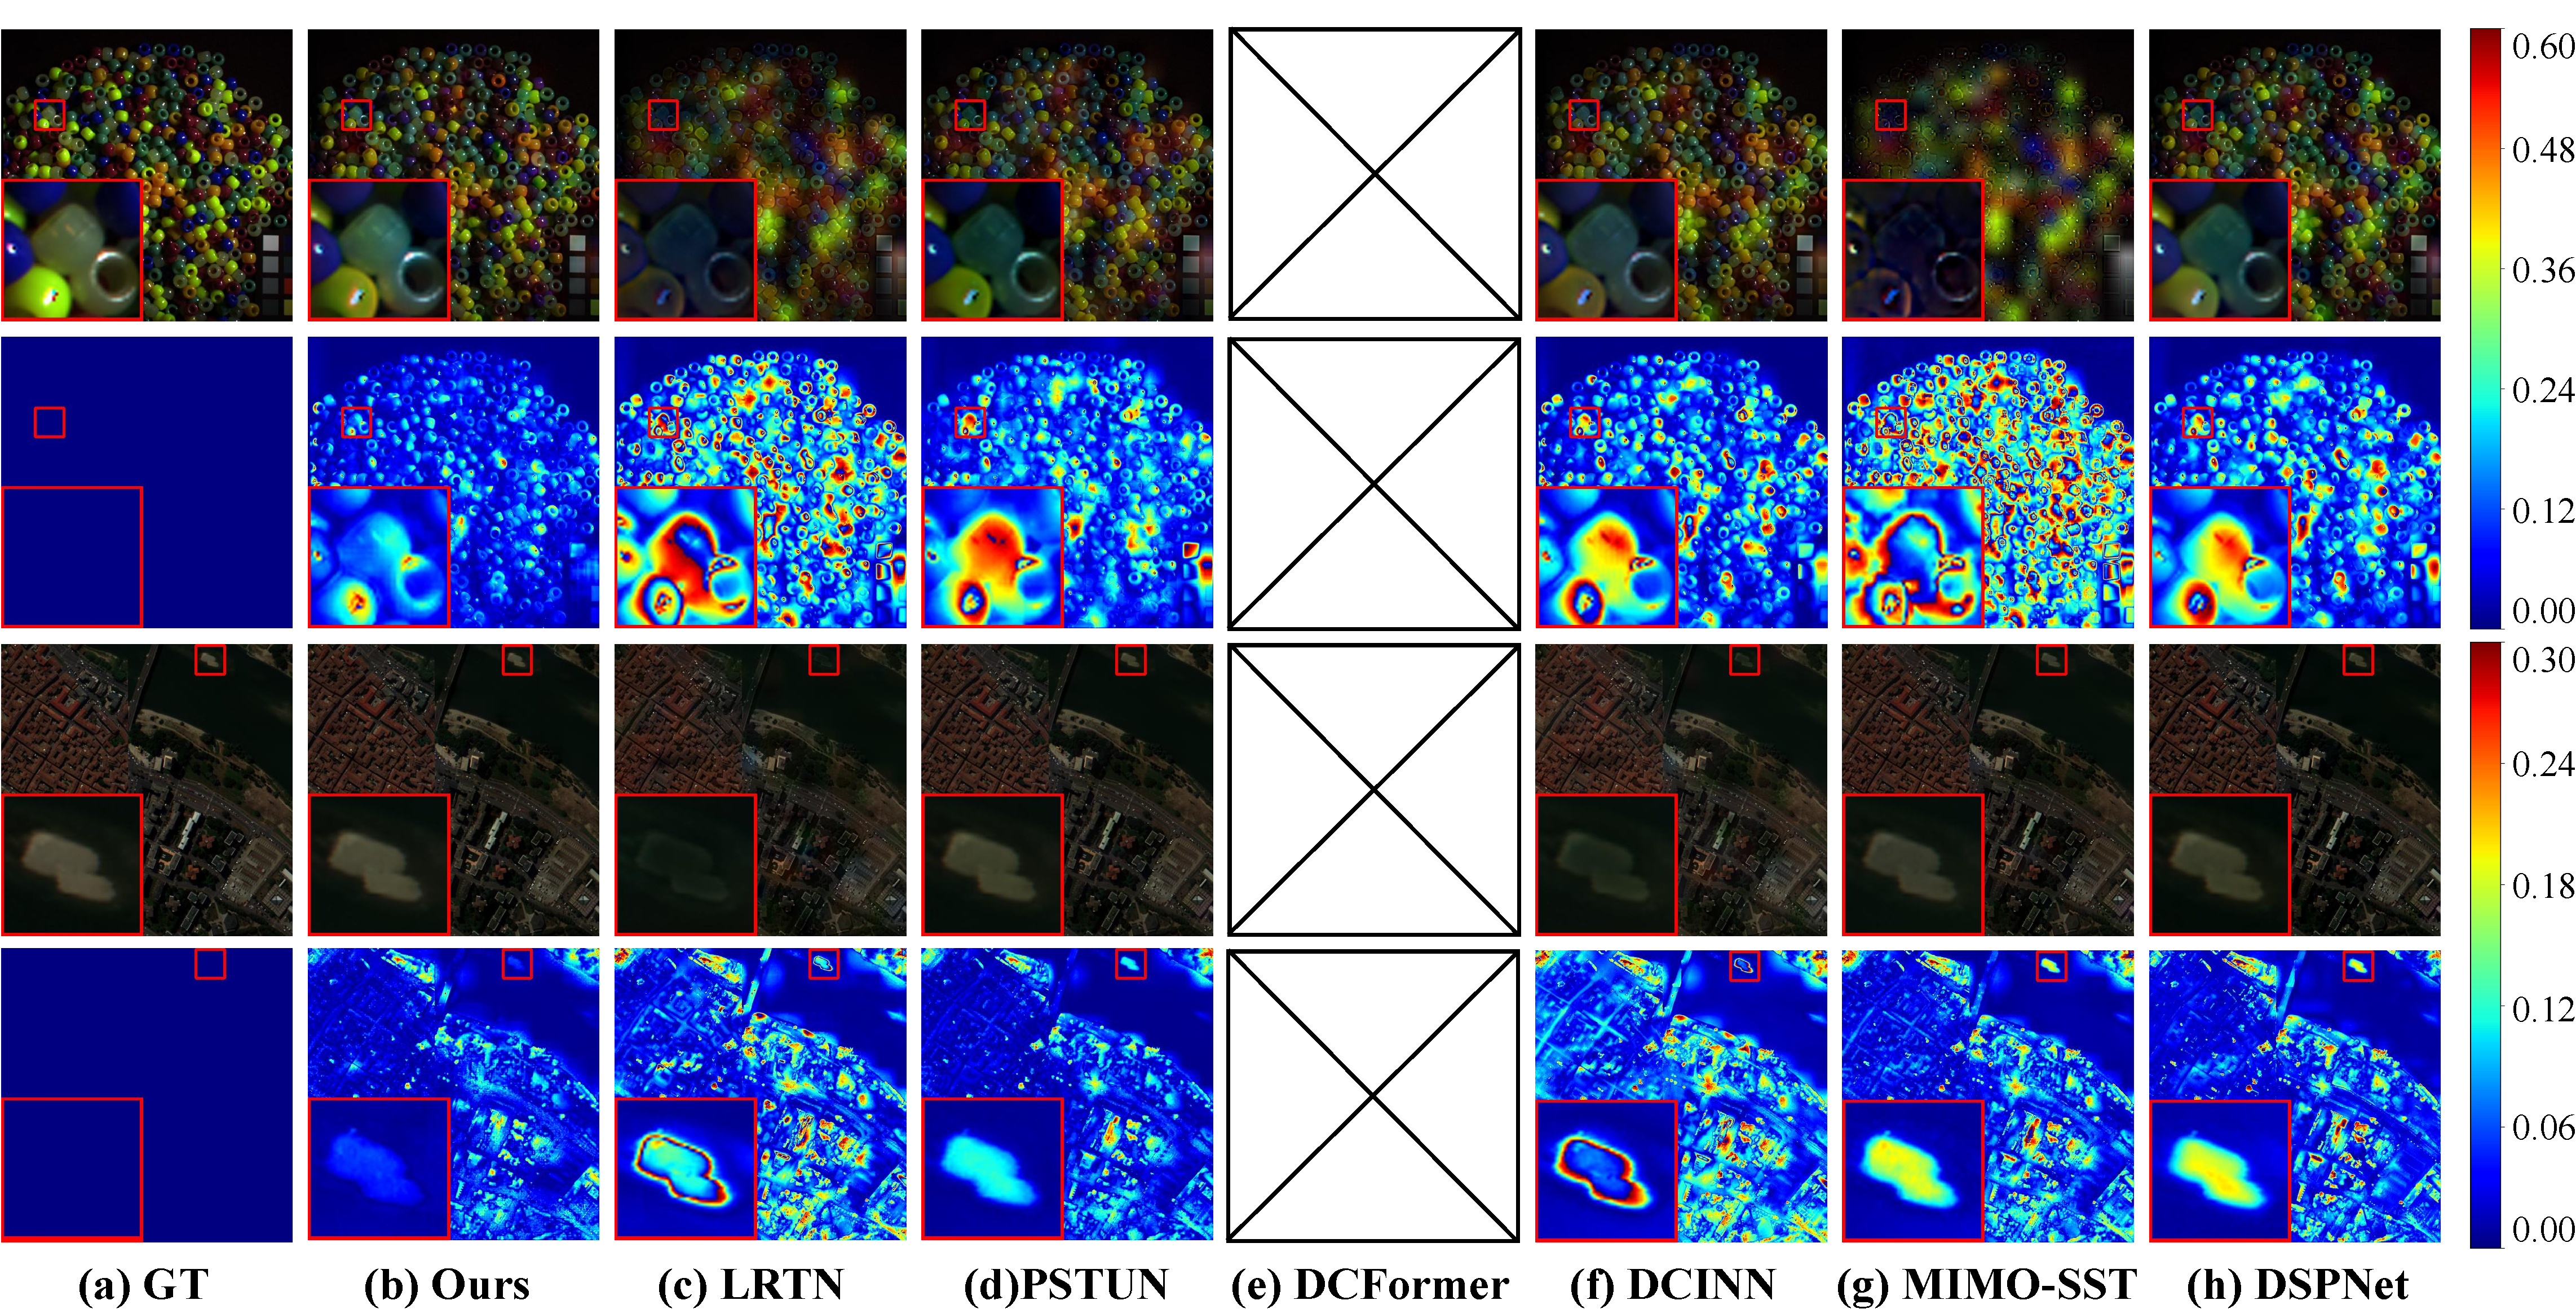
\includegraphics[width=0.95\textwidth]{Figs/fig_cave_paviac31.pdf}
    \caption{Qualitative comparison on the \textbf{CAVE} (top rows) and \textbf{PaviaC} (bottom rows) datasets at the unseen \textbf{$\times 32$ scale}. The red boxes highlight close-up details, and the even rows display the corresponding error maps. Our SSA model exhibits superior detail recovery and minimal reconstruction error compared to SOTA methods, which suffer from significant blurriness at this extreme scale.}
    \label{fig:cave_paviac_vis}
\end{figure*}
\begin{figure*}
    \centering
    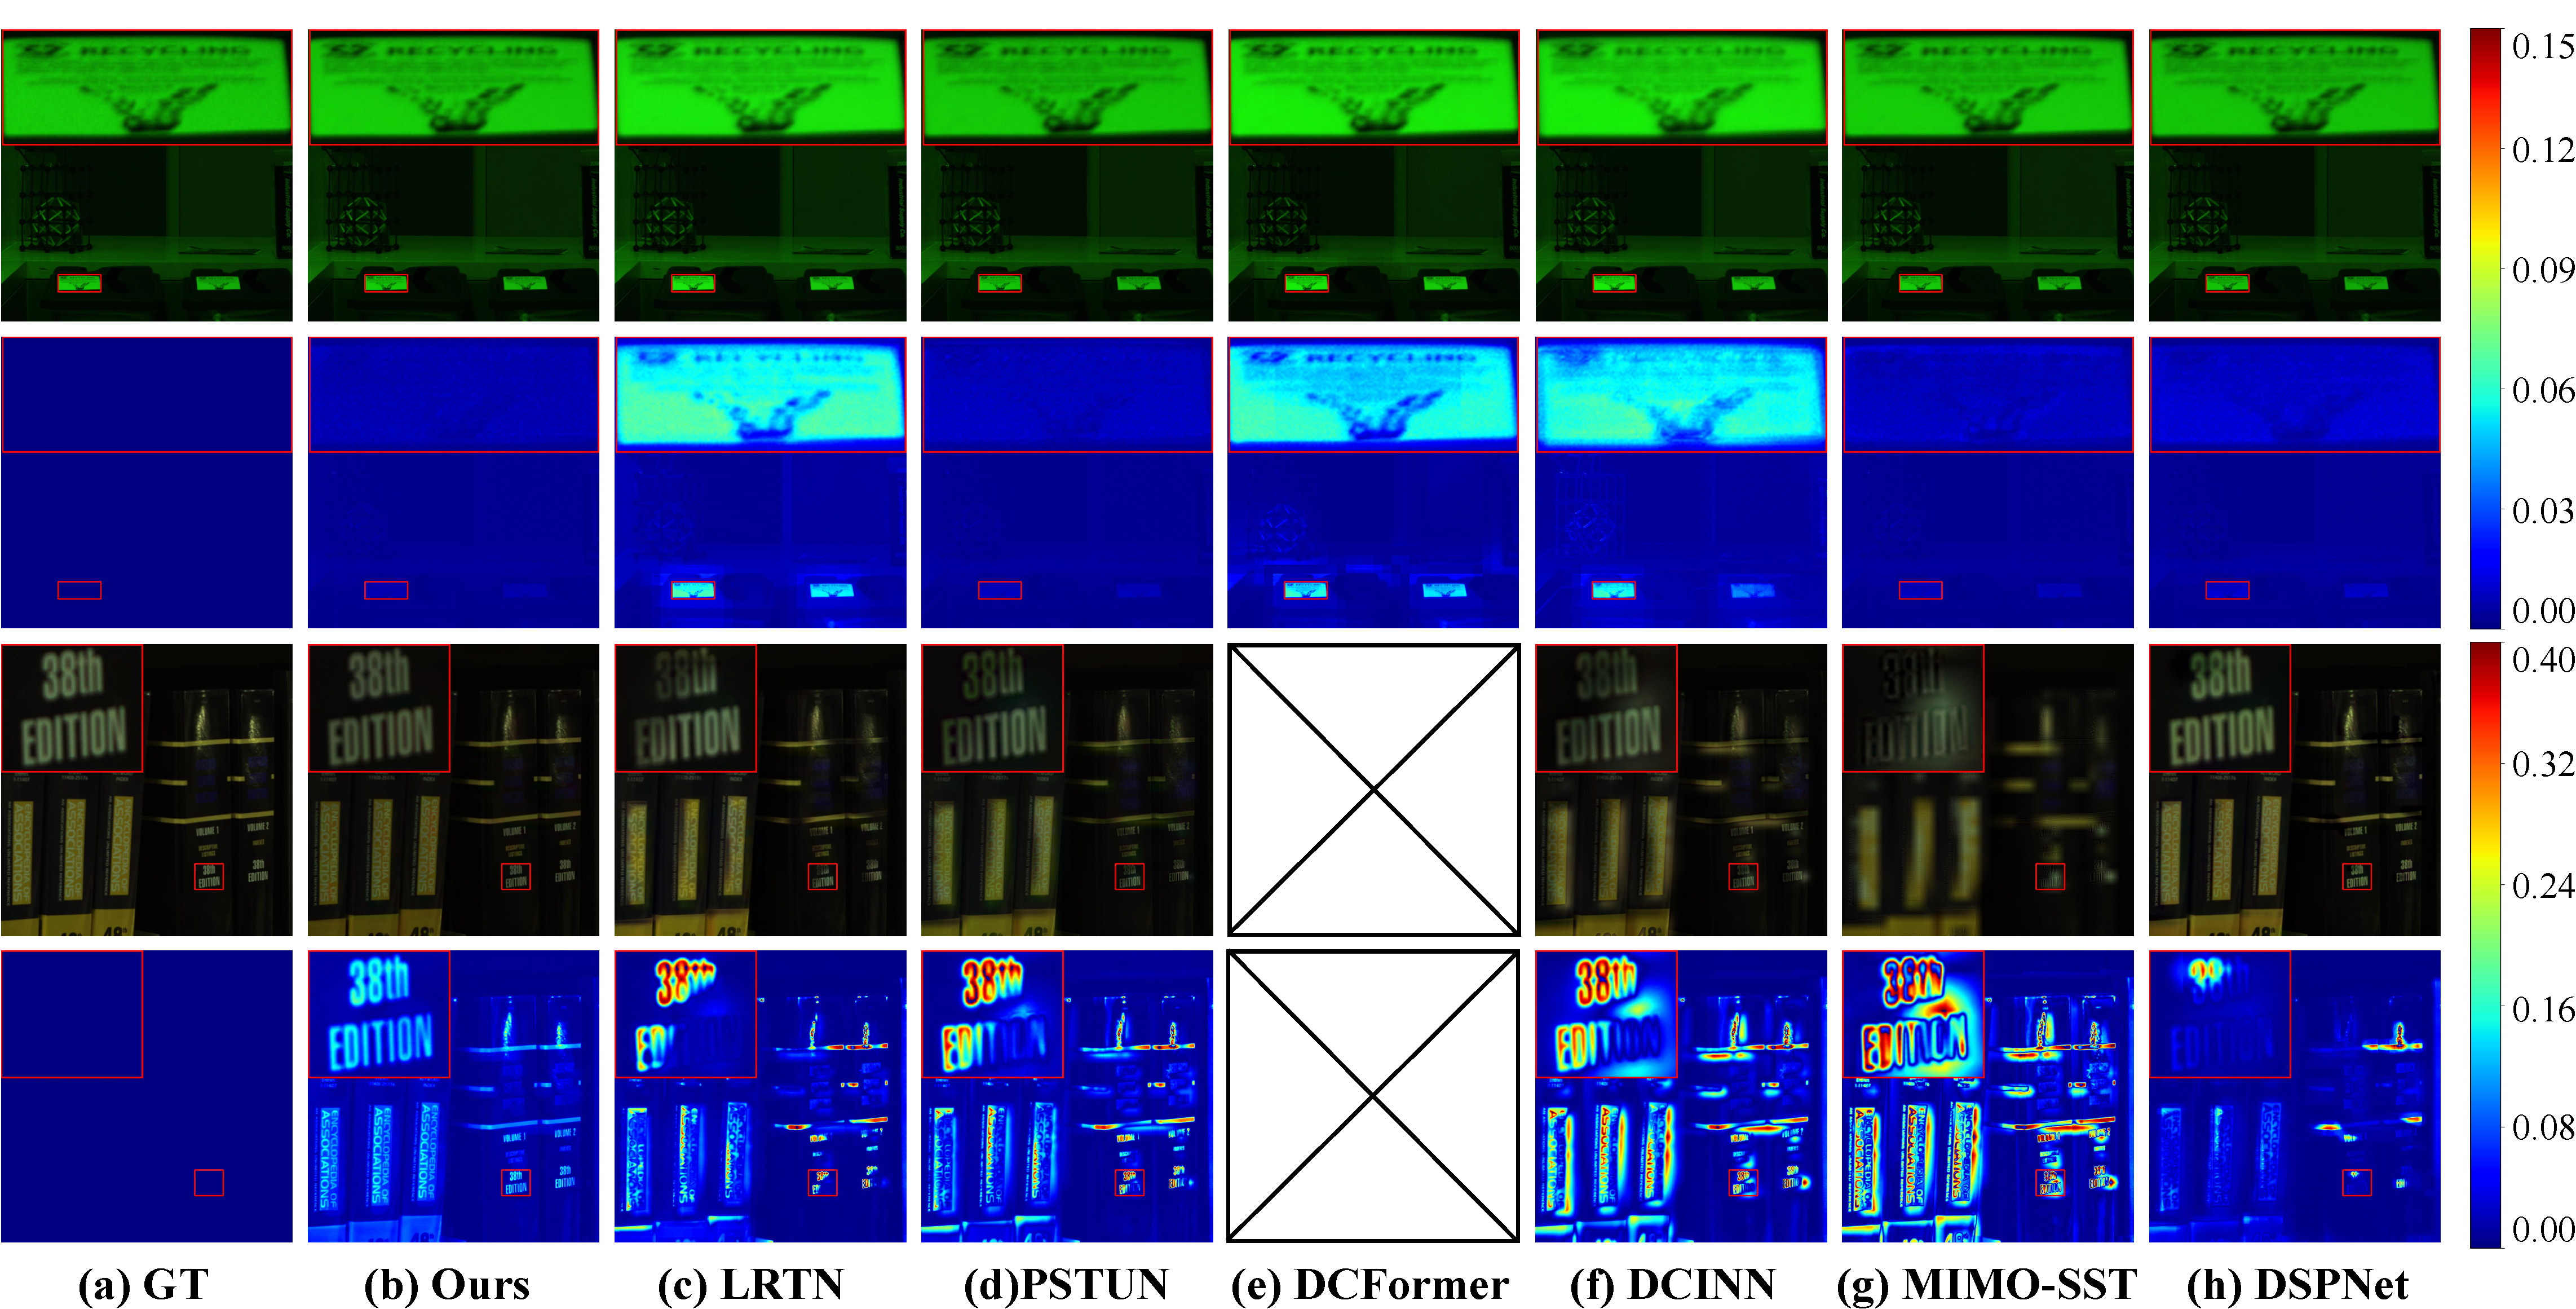
\includegraphics[width=0.95\textwidth]{Figs/fig_harvard.pdf}
    \caption{Visual comparison on the \textbf{Harvard} dataset. The top two rows correspond to the in-distribution $\times 4$ scale, and the bottom two rows correspond to the unseen $\times 32$ scale. Our method preserves sharp textual details (see zoom-in) even at large magnification factors.}
    \label{fig:harvard_vis}
\end{figure*}

\begin{figure*}
    \centering
    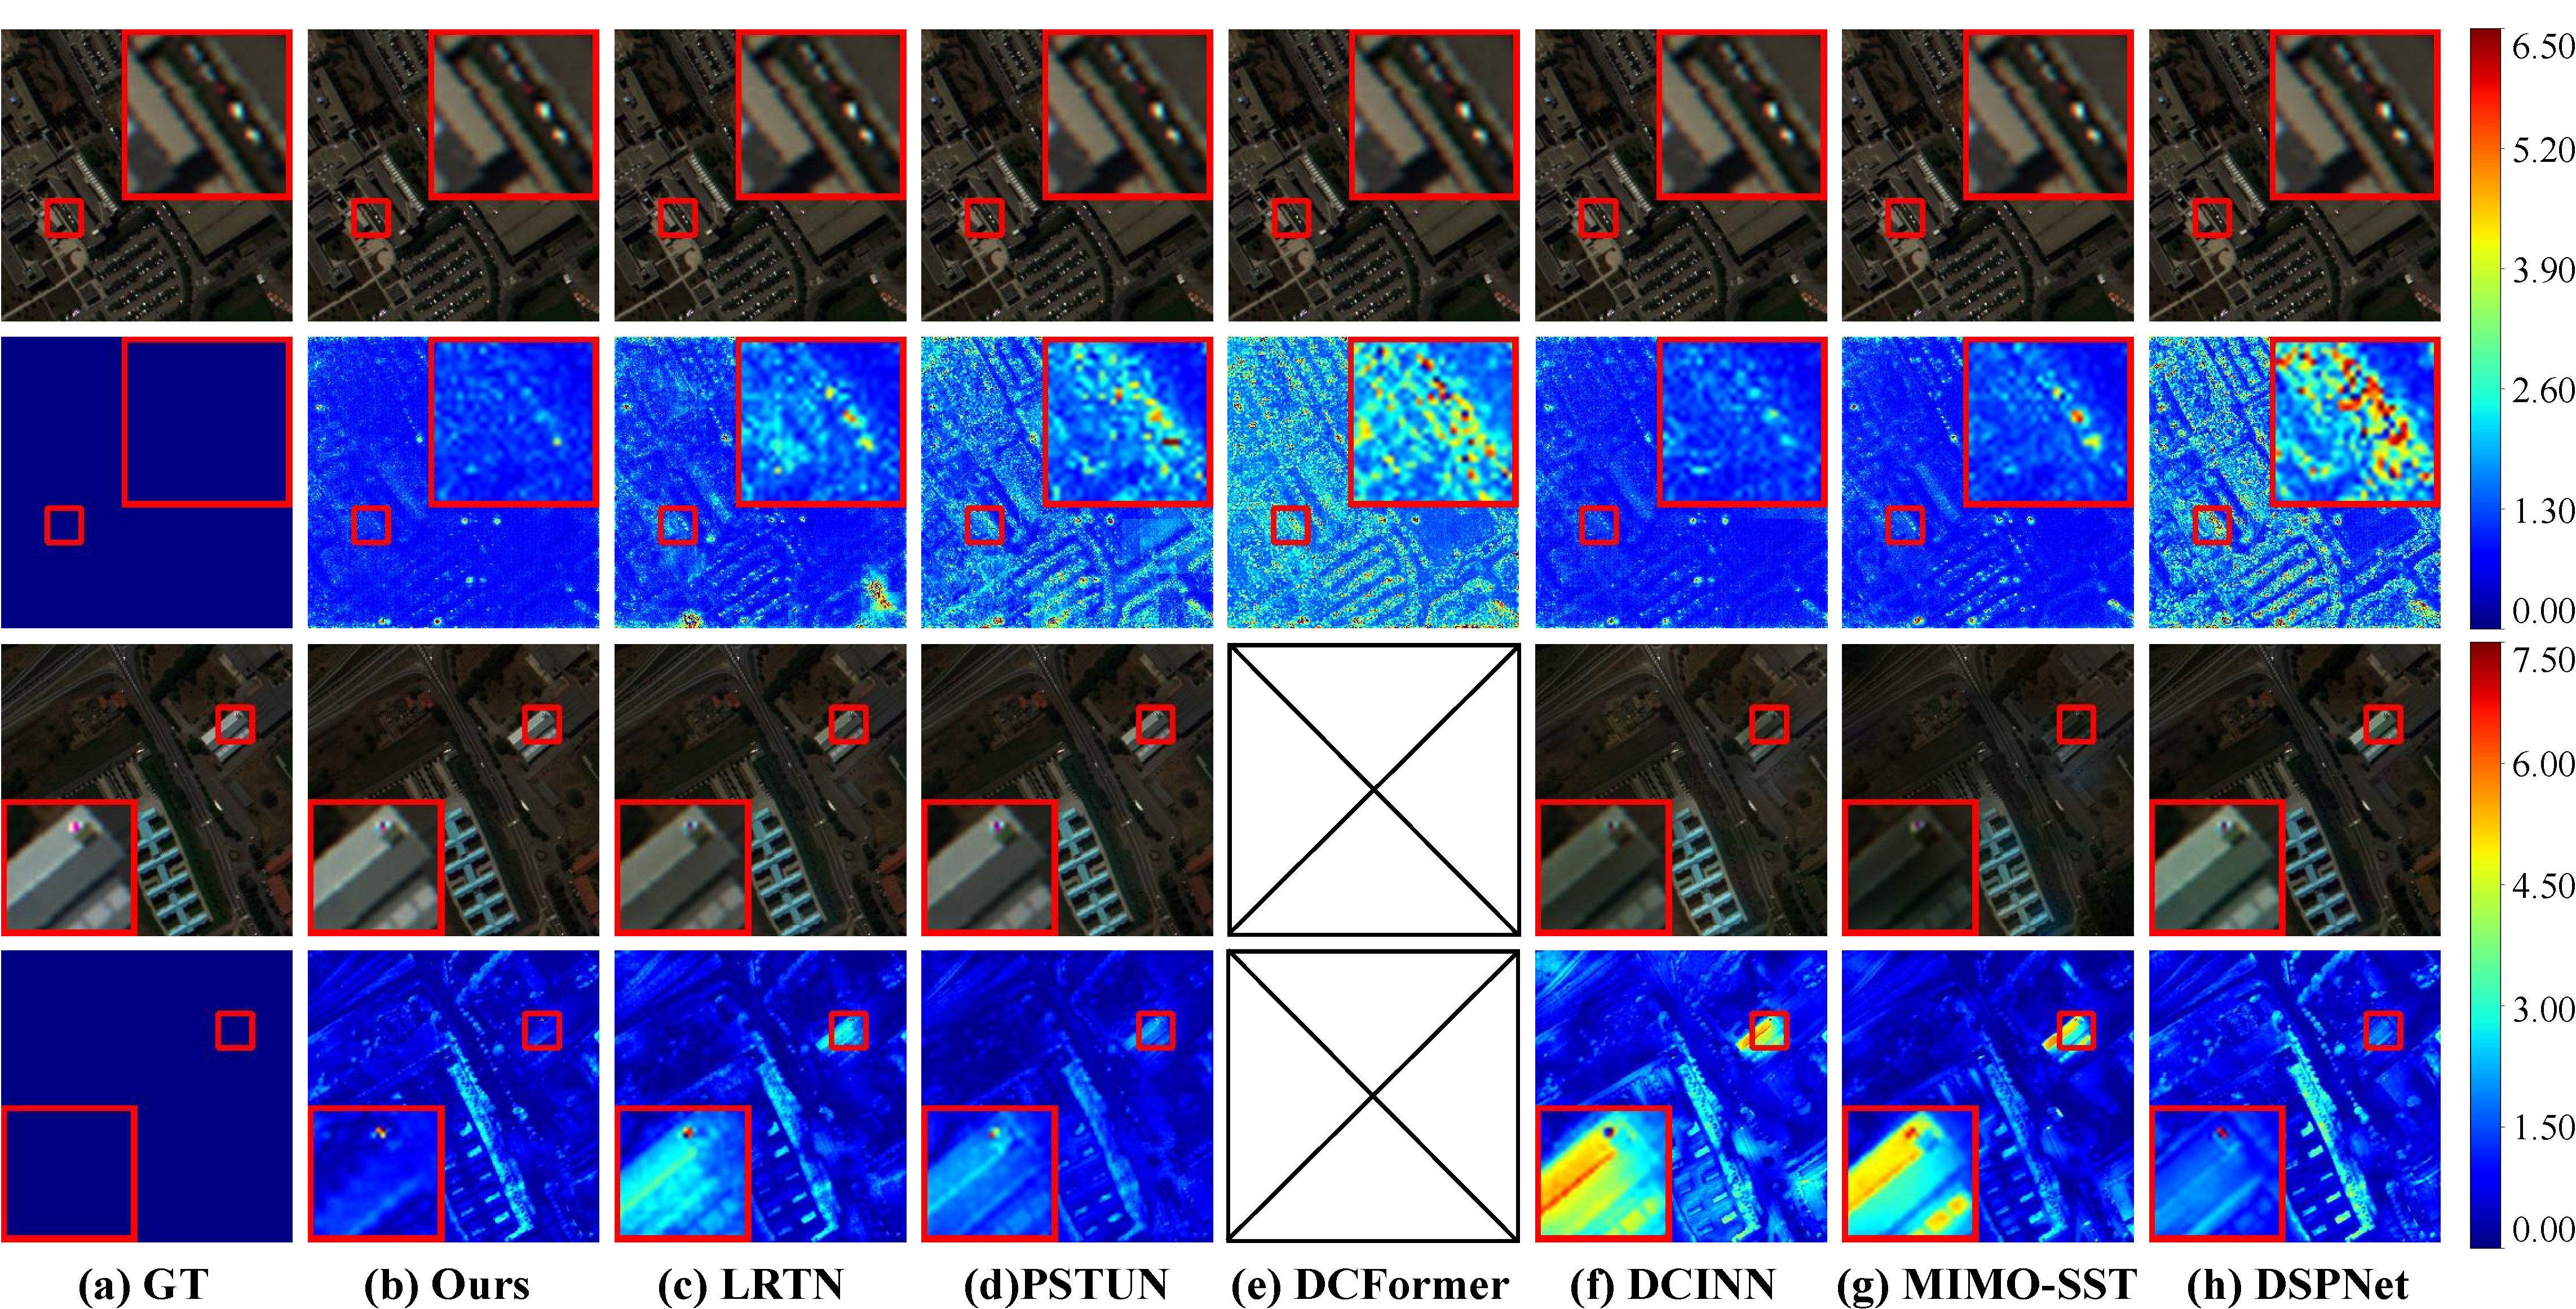
\includegraphics[width=0.95\textwidth]{Figs/fig_paviau.pdf}
    \caption{Visual comparison on the \textbf{PaviaU} dataset across varying scales. The top two rows show the results at the training scale ($\times 4$), while the bottom two rows display the out-of-distribution scale ($\times 32$). For each scale, we present the fused image and its corresponding error map. Note that DCFormer~\cite{wu2025fully} fails to support the arbitrary $\times 32$ scale (indicated by crossed boxes).}
    \label{fig:paviau_vis}
\end{figure*}
\begin{figure*}
    \centering
    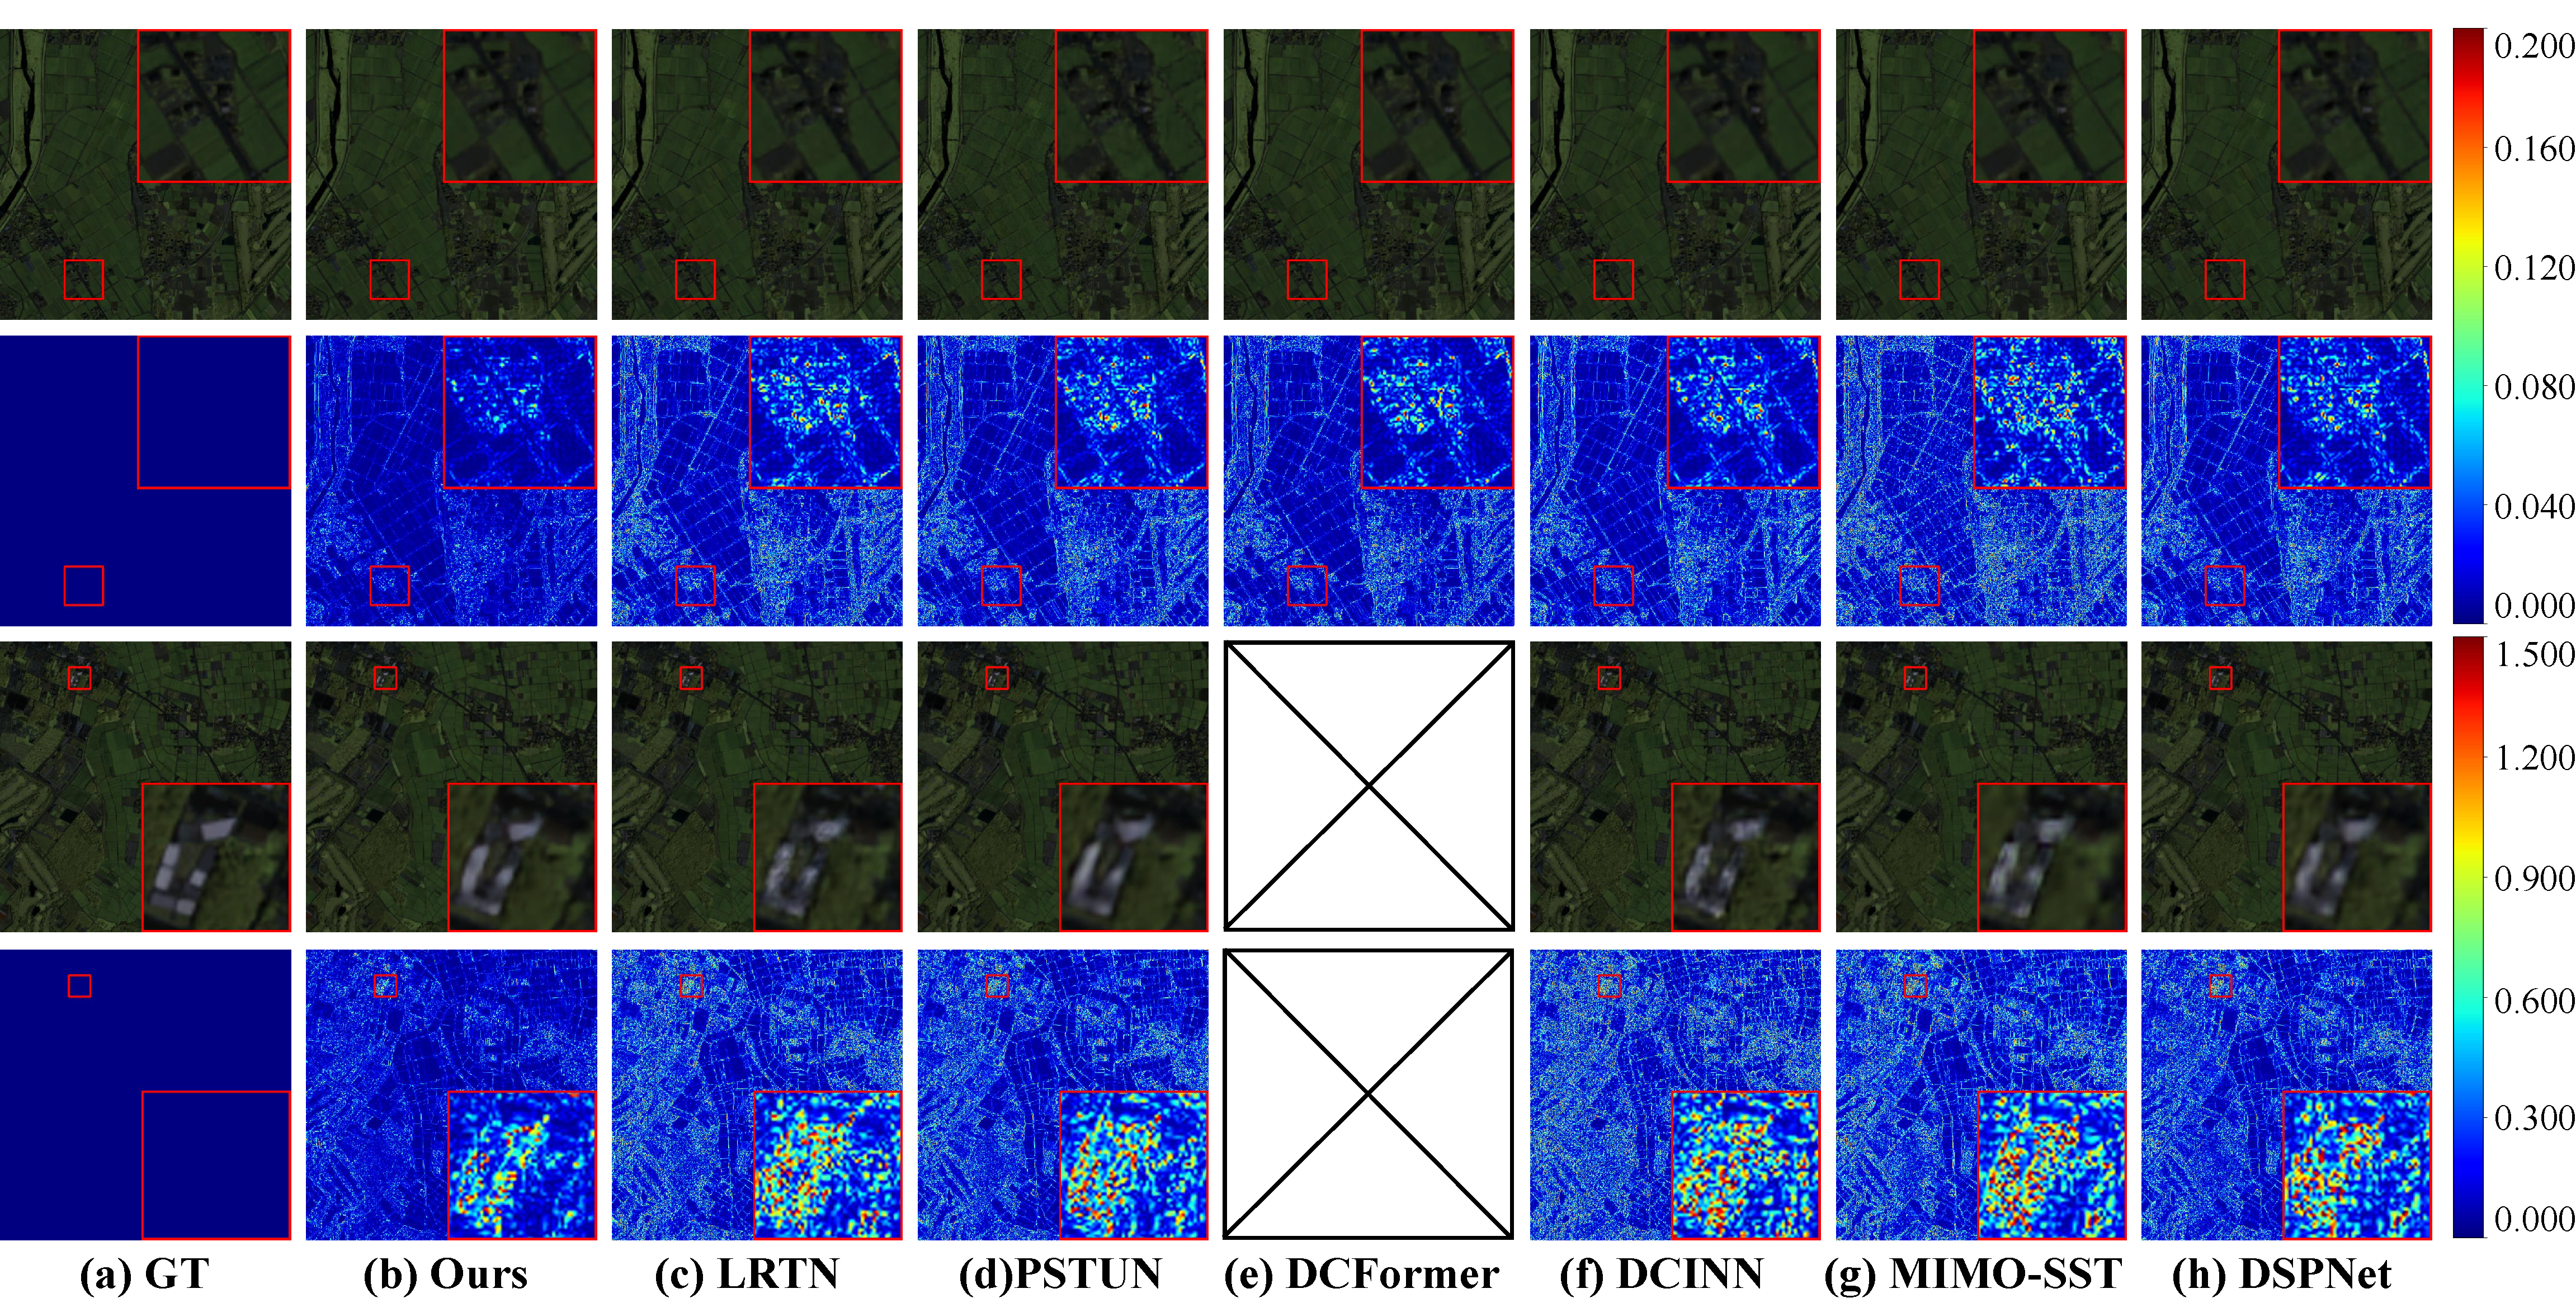
\includegraphics[width=0.95\textwidth]{Figs/fig_chikusei.pdf}
    \caption{Visual comparison on the \textbf{Chikusei} dataset. Top two rows: $\times 4$ scale; Bottom two rows: $\times 32$ scale. The error maps (blue indicates low error) demonstrate that our model generalizes well to large-scale remote sensing scenes with varying spatial resolutions.}
    \label{fig:chikusei_vis}
\end{figure*}
\begin{figure*}
    \centering
    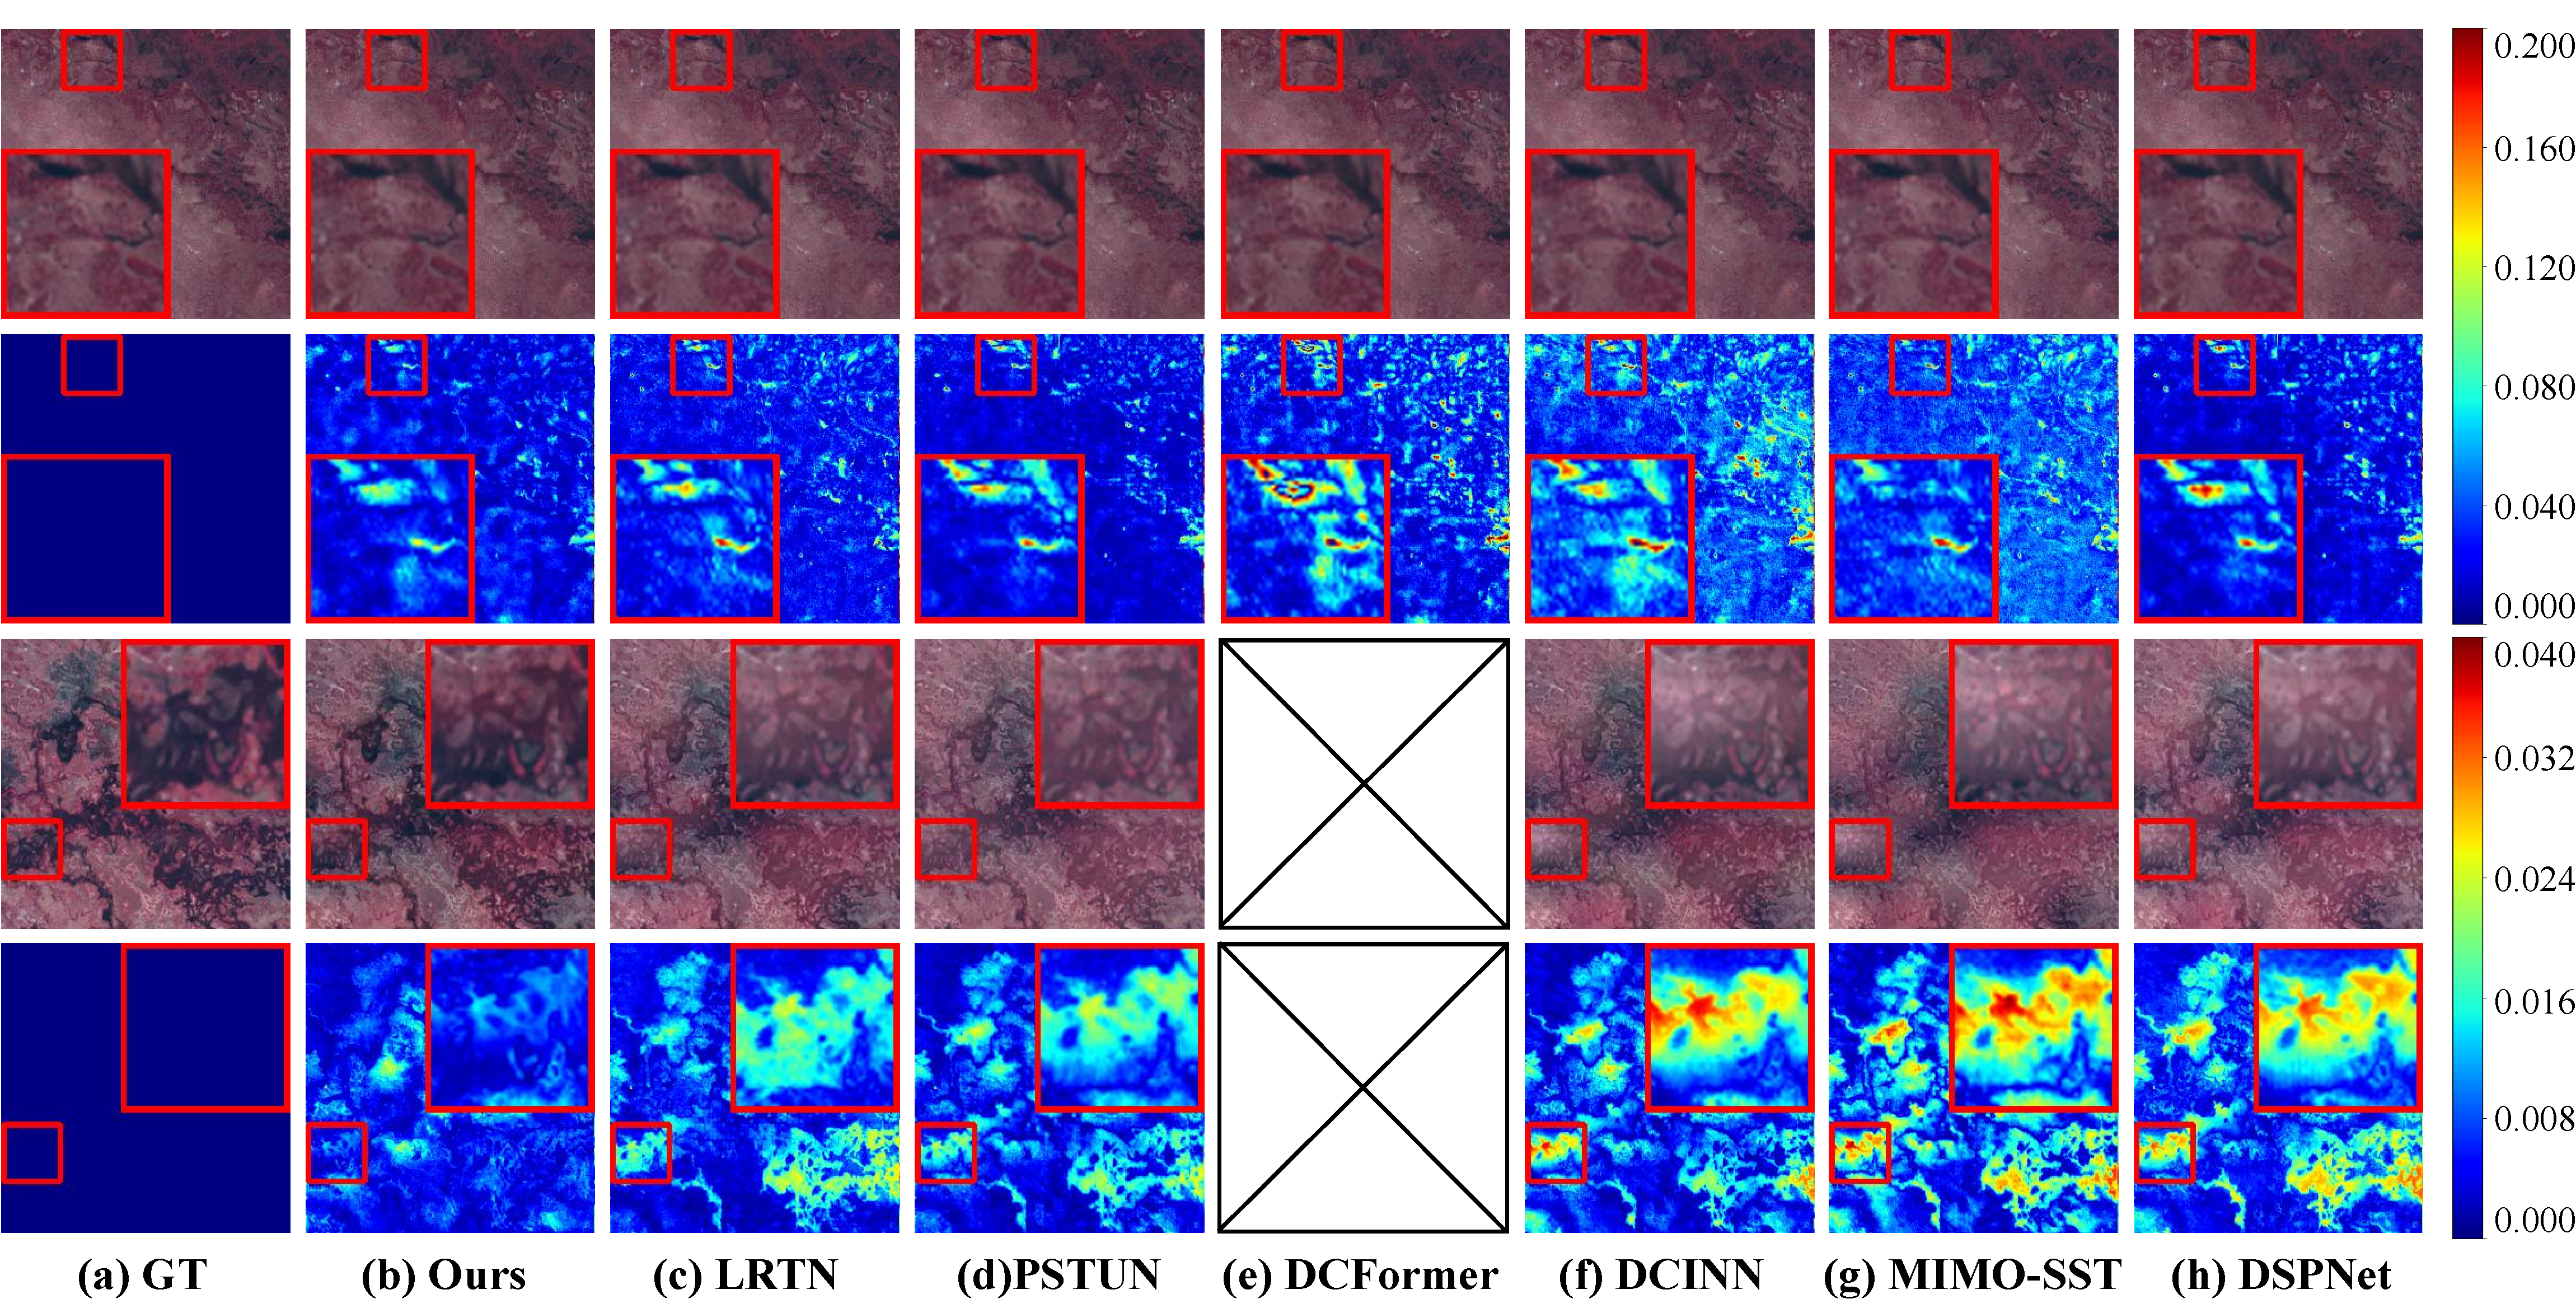
\includegraphics[width=0.95\textwidth]{Figs/fig_botswana.pdf}
    \caption{Visual comparison on the \textbf{Botswana} dataset. Top two rows: $\times 4$ scale; Bottom two rows: $\times 32$ scale. Our approach maintains spectral and spatial consistency better than comparison methods, which often show high-energy residuals (red/yellow) at large upscaling factors.}
    \label{fig:botswana_vis}
\end{figure*}
\begin{figure*}
    \centering
    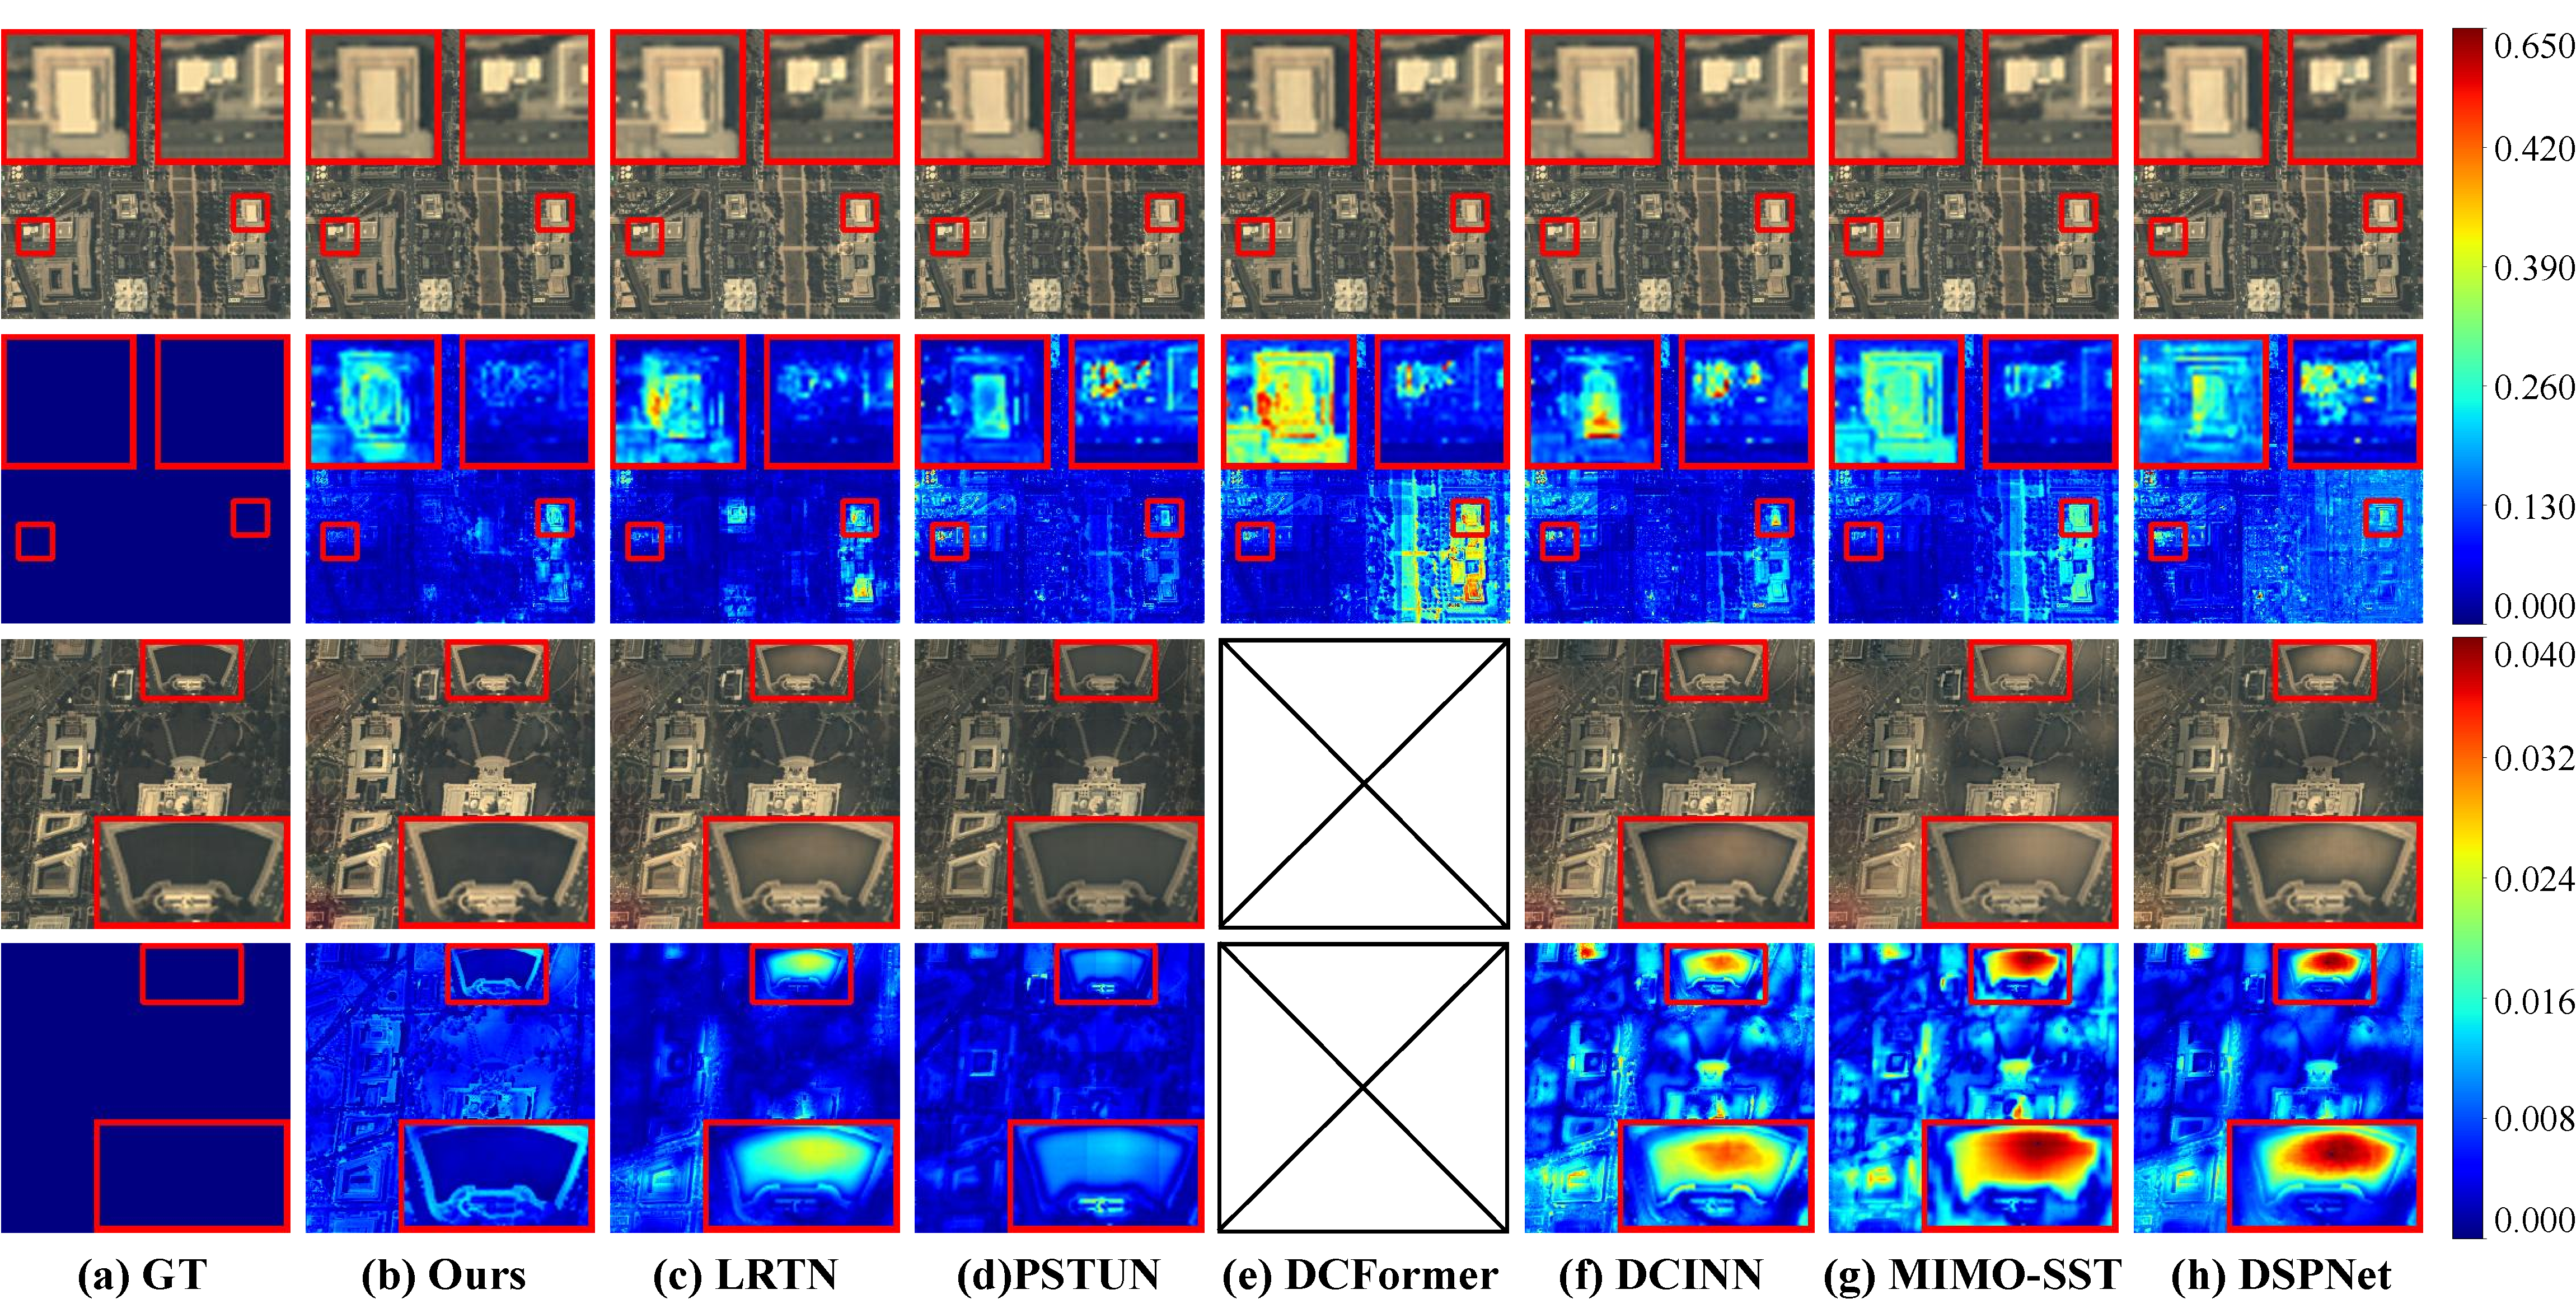
\includegraphics[width=0.95\textwidth]{Figs/fig_washingtondc.pdf}
    \caption{Visual comparison on the \textbf{WashingtonDC} dataset. Top two rows: $\times 4$ scale; Bottom two rows: $\times 32$ scale. Despite the high band count (191 bands), our unified model robustly reconstructs spatial details across different scaling factors without model retraining.}
    \label{fig:washingtondc_vis}
\end{figure*}

